\chapter{spazi di funzioni}

%%%%%%%%%%%%%%%%%%%%%%%%
%%%%%%%%%%%%%%%%%%%%%%%%

\begin{figure}
  \centering
  \begin{tikzpicture}[node distance=2cm]
    \draw node at (0,0)[name=insieme]{insieme};
    \draw node at (-1,-1)[name=sv]{sp. vettoriale};
    \draw node at (-1,-3)[name=sn]{sp. normato};
    \draw node at (-1,-5)[name=euclideo]{sp. euclideo};
    \draw node at (2,-1)[name=st]{sp. topologico};
    \draw node at (2,-2)[name=sm]{sp. metrico};
    \draw node at (2,-3.5)[name=completo]{sp. completo};
    \draw node at (1,-4.5)[name=banach]{Banach};
    \draw node at (1,-6)[name=hilbert]{Hilbert};
    \draw[->](sv) -- (insieme);
    \draw[->](st) -- (insieme);
    \draw[->](sn) -- (sv);
    \draw[->](sm) -- (st);
    \draw[->](euclideo) -- (sn);
    \draw[->](hilbert) -- (euclideo);
    \draw[->](hilbert) -- (banach);
    \draw[->](banach) -- (completo);
    \draw[->](completo) -- (sm);
    \draw[->](sn) -- (sm);
    \draw[->](banach) -- (sn);

    \begin{scope}[black!40]
    \draw node at (-2,0)[name=insiemeT]{$\in,\subset,\cup$};
    \draw (insiemeT) -- (insieme);
    \draw node at (-3,-1)[name=svT]{$+,\cdot$};
    \draw (svT) -- (sv);
    \draw node at (-3,-3)[name=snT]{$\abs{v}$};
    \draw (snT) -- (sn);
    \draw node at (-3,---5)[name=euclideoT]{$\langle v,w\rangle$};
    \draw (euclideoT) -- (euclideo);
    \draw node at (5,0)[name=stT]{$\lim, \stackrel\circ A, \bar A$};
    \draw (stT) -- (st);
    \draw node at (5,-1.75)[name=smT]{$d(x,y)$, Lip};
    \draw (smT) -- (sm);
    \end{scope}

    \begin{scope}[black!75]
    \draw node at (5,-1)[name=Rbar,left]{$\bar \RR$};
    \draw[->](Rbar) -- (st);
      \draw node at (5,-2.5)[name=Q,left]{$\QQ$};
      \draw[->](Q) -- (sm);
      \draw node at (5,-4)[name=Sn,left]{$\mathbb S^n$};
      \draw[->](Sn) -- (completo);
      \draw node at (4.5,-5)[name=Cn,left]{$\mathcal C^n$, $L^p$, $\ell^p$};
      \draw[->](Cn) -- (banach);
      \draw node at (4,-6.5)[name=L2,left]{$L^2$, $\ell^2$};
      \draw[->](L2) -- (hilbert);
      \draw node at (1,-7)[name=Rn]{$\RR^n$};
      \draw[->](Rn) -- (hilbert);
    \end{scope}
  \end{tikzpicture}
\caption{Strutture matematiche che astraggono lo spazio $\RR^n$.
La freccia nera significa: ``è un'',
la freccia scura: ``è un esempio di'',
la linea chiara: ``è una operazione tipica di''.}
\label{fig:spazi}
\end{figure}

L'astrazione è una attività tipica della matematica. I risultati che abbiamo
visto fin'ora riguardano per lo più lo spazio $\RR$ dei numeri reali
e in parte lo spazio $\CC$ dei numeri complessi.
E' però evidente che molti di questi risultati si estendono ad altre situazioni
più generali. Identificare le proprietà fondamentali che stanno alla base
di un teorema è forse l'attività più importante svolta dalla matematica.
Tipicamente l'identificazione di queste proprietà oltre a generalizzare
un risultato ne rende anche più semplice la dimostrazione.
Infatti una volta identificate le ipotesi minime del teorema
gli strumenti a nostra disposizione pure si riducono e sarà più facile
capire quali andranno utilizzati.
D'altra parte non potremo portare all'estremo questo tentativo di generalizzazione
in quanto ci si accorge presto che la fauna composta dagli spazi che vanno via
via a coprire tutte le possibili tipologie diventa subito enorme e avere
in mente tutte le definizioni diventa troppo oneroso.

Si veda la figura~\ref{fig:spazi} per avere un quadro relazionale
degli spazi che andremo ora ad introdurre.
Gli insiemi sono dati per noti (si vedano gli appunti di logica \cite{appunti_logica}).
Anche gli spazi vettoriali (algebra lineare) li diamo per noti, in quanto sono usualmente oggetto
del corso di geometria.
Gli spazi topologici verranno solamente accennati in quanto non saranno direttamente
utili ai nostri scopi e una trattazione completa richiederebbe molto tempo.
Per lo stesso motivo mancano completamente da questa classificazione anche altri
spazi molto rilevanti (ad esempio i gruppi e le varietà differenziali).


\begin{definition}[spazio metrico]
\mymark{**}
\label{def:distanza}
Diremo che $d\colon X\times X\to\RR$ è una \myemph{distanza} su $X$
se per ogni $x,y,z\in X$ valgono le seguenti proprietà
\begin{enumerate}
\item
  $d(x,y)\ge 0$ (positività);
\item
  $d(x,y)\le d(x,z) + d(z,y)$ (disuguaglianza triangolare);
\item
  $d(x,y)=0$ se e solo se $x=y$ (separazione);
\item
  $d(x,y) = d(y,x)$ (simmetria).
\end{enumerate}

Se $d$ è una distanza
diremo che $X$ è uno
\emph{spazio metrico}
\mynote{spazio metrico}%
\index{spazio!metrico}%
(metrizzato da $d$).
\end{definition}

Osserviamo che dalle disuguaglianze triangolari:
\[
  d(x,z) \le d(x,y) + d(y,z), \qquad
  d(y,z) \le d(x,y) + d(x,z)
\]
si ottiene la \emph{disuguaglianza triangolare inversa}:
\mynote{disuguaglianza triangolare inversa}
\index{disuguaglianza!triangolare!inversa}
\[
  d(x,y) \ge \abs{d(x,z) - d(y,z)}.
\]

\begin{definition}[convergenza]
\mymark{*}
Se $x_n \in X$ è una successione di punti di uno spazio metrico $X$
e $x\in X$ diremo che $x_n$ converge a $x$ e scriveremo
\[
  x_n \to x
\]
se $d(x_n,x)\to 0$ per $n\to +\infty$.
\end{definition}

Si noti che l'usuale convergenza in $\RR$ non è altro
che la convergenza di $\RR$
visto come spazio metrico con la distanza euclidea $d(x,y) = \abs{x-y}$.

Con l'artificio $d(x_n,y_n) - d(x,y) = d(x_n,y_n) - d(x_n,y) + d(x_n,y) - d(x,y)$
e utilizzando la disuguaglianza triangolare inversa si può
facilmente risolvere il seguente.

\begin{exercise}[continuità della distanza]
Dimostrare che se $x_n\to x$ e $y_n\to y$
allora $d(x_n,y_n) \to d(x,y)$.
\end{exercise}

\begin{definition}[spazio normato]
\mymark{*}
\label{def:norma}
Sia $V$ uno spazio vettoriale sul campo $\RR$.
Una funzione $\phi \colon V\to \RR$ si
dice essere una \myemph{norma} su $V$ se
per ogni $v,w\in V$ e per ogni $\lambda \in \RR$
valgono le seguenti proprietà:
\begin{enumerate}
\item
  $\phi(v) \ge 0$ (positività);
\item
  $\phi(\lambda v) = \abs{\lambda} \cdot \phi(v)$ (omogeneità e simmetria);
\item
  $\phi(v+w) \le \phi(v) + \phi(w)$
  (disuguaglianza triangolare);
\item
  $\phi(v)=0$ se e solo se $v=0$ (separazione).
\end{enumerate}

Se $\phi$ è una norma su $V$ diremo che
$V$
è uno spazio vettoriale \myemph{normato} da $\phi$.

Se $\phi$ è una norma la funzione $d(v,w) = \phi(v-w)$
è chiaramente una distanza che si chiama
\emph{distanza indotta}
\mynote{distanza indotta}
\index{distanza!indotta}
da $\phi$.
In particolare ogni spazio normato è anche uno spazio metrico rispetto alla
distanza indotta dalla norma.
%Inoltre la disuguaglianza triangolare
%assicura che la norma $\phi\colon V\to \RR$ risulta essere una %+funzione continua.
\end{definition}

Usualmente si utilizzano le notazioni $\abs{v}$ o $\Abs{v}$ per indicare
una norma $\phi(v)$.

Visto che uno spazio normato è anche uno spazio metrico, negli spazi
normati è definita una convergenza. E' facile verificare che la norma risulta
essere continua rispetto a tale convergenza, nel senso che se $v_k \to v$
(ovvero $\phi(v_k-v)\to 0$) allora $\phi(v_k)\to \phi(v)$.

\begin{definition}[spazio euclideo]
\label{def:prodotto_scalare}
Sia $V$ uno spazio vettoriale sul campo $\RR$.
Una funzione $b\colon V\times V \to \RR$ si dice
essere un \myemph{prodotto scalare definito positivo} su $V$ se
$b$ è una forma bilineare, simmetrica e definita
positiva, ovvero se
per ogni $u,v,w\in V$ e per ogni $\lambda, \mu \in \RR$
valgono le seguenti proprietà:
\begin{enumerate}
\item $b(v,v) \ge 0$ (positività);
\item $b(\lambda u + \mu v, w) = \lambda b(u,w) + \mu b(v,w)$
e $b(u,\lambda v+ \mu w) = \lambda b(u,v) + \mu b(u,w)$
(bilinearità);
\item $b(v,w) = b(w,v)$ (simmetria);
\item $b(v,v) = 0$ se e solo se $v=0$ (non degenerazione).
\end{enumerate}

Se $b$ è un prodotto scalare definito positivo su $V$ diremo che $V$ è uno
spazio \emph{euclideo} (con prodotto scalare $b$).

Usualmente si utilizzano le notazioni $v\cdot w$, $(v,w)$, $\langle v,w\rangle$
o $\langle v \vert w\rangle$ per denotare un prodotto scalare $b(v,w)$.
\end{definition}

Se $b$ è un prodotto scalare definito positivo su $V$ il teorema seguente ci garantisce che
che la funzione $\phi(v) = \sqrt{\langle v,v\rangle}$ è una norma su $V$.

Dunque uno spazio euclideo ha, in modo naturale, una struttura di spazio
normato e di spazio metrico.

\begin{theorem}[proprietà del prodotto scalare]
\label{th:spazio_euclideo}%
Sia $V$ uno spazio euclideo con prodotto scalare (definito positivo) $\langle v, w\rangle$.
Si definisca $\abs{v} = \sqrt{\langle v,v\rangle}$.
Allora $\abs{v}$ è una norma su $V$
e per ogni $v,w\in V$ valgono le seguenti proprietà:
\begin{enumerate}
\item \myemph{sviluppo del binomio}
\[
  \abs{v+w}^2 = \abs{v}^2 + 2 \langle v,w\rangle + \abs{w}^2;
\]
\item \myemph{teorema!di Pitagora}
\index{Pitagora!teorema}%
\begin{equation}\label{eq:Pitagora}
  \langle v,w\rangle=0 \implies \abs{v+w}^2 = \abs{v}^2 + \abs{w}^2;
\end{equation}
\item \myemph{disuguaglianza di Young}
\index{Young!disuguaglianza di}%
\begin{equation}\label{eq:Young}
  \langle v,w\rangle \le \frac{\abs{v}^2 + \abs{w}^2}{2};
\end{equation}
\item \myemph{disuguaglianza!di Cauchy-Schwarz}
\index{Cauchy-Schwarz!disuguaglianza di}%
\begin{equation}\label{eq:Cauchy_Schwarz}
   \langle v,w \rangle \le \abs{v} \cdot \abs{w};
\end{equation}
\item \myemph{proprietà del parallelogramma}
\index{parallelogramma!proprietà del}
\begin{equation}\label{eq:parallelogramma}
  \abs{v+w}^2 + \abs{v-w}^2 = 2 \abs{v}^2 + 2\abs{w}^2;
\end{equation}
\item \emph{continuità}
\[
  \text{se $v_k\to v$ e $w_k\to w$ allora
  $\langle v_k,w_k\rangle \to \langle v,w \rangle$}.
\]
\end{enumerate}
\end{theorem}
%
\begin{proof}
Osserviamo innanzitutto che $\abs{v}$ è ben definita per ogni $v\in V$
in quanto il prodotto scalare $\langle v,v\rangle$ per definizione non è mai negativo.
Allora in generale si ha, sfruttando la bilinearità,
l'usuale sviluppo del quadrato del binomio:
\begin{align*}
  \abs{v+w}^2
  &= \langle v+w, v+w\rangle
  = \langle v+w, v\rangle + \langle v+w, w\rangle \\
  &= \langle v,v\rangle + 2\langle v,w \rangle + \langle w,w\rangle
  = \abs{v}^2 + 2\langle v,w \rangle + \abs{w}^2.
\end{align*}
Il teorema di Pitagora segue immediatamente.
Ma allora si ottiene facilmente la disuguaglianza di Young:
\[
  0 \le \abs{v-w}^2 = \abs{v}^2 + \abs{w}^2 - 2 \langle v,w\rangle
\]
e la proprietà del parallelogramma:
\[
  \abs{v+w}^2 + \abs{v-w}^2
  = \abs{v}^2 + 2\langle v,w \rangle + \abs {w}^2
    + \abs{v}^2 - 2\langle v,w\rangle + \abs{w}^2.
\]
Ora se $\abs{v}=\abs{w}=1$ la disuguaglianza di Young ci dice che
\[
  \langle v,w \rangle \le 1.
\]
Ma allora per ogni $v\neq 0$ e $w \neq 0$ si ottiene
la disuguaglianza di Cauchy-Schwarz:
\[
\frac{\langle v,w\rangle}{\abs{v}\cdot \abs{w}}
 = \langle \frac{v}{\abs{v}} , \frac{w}{\abs{w}}\rangle
 \le 1.
\]
Se invece $v=0$ o $w=0$ la disuguaglianza di Cauchy-Schwarz è ovvia in quanto
per ogni $u\in V$ si ha
$\langle 0, u\rangle = \langle u,0\rangle = 0$ per bilinearità.

Per quanto riguarda la continuità
ricordiamoci che $v_k \to v$ significa $\abs{v_k-v}\to 0$.
Possiamo allora scrivere
\begin{align*}
  \langle v_k,w_k\rangle - \langle v,w\rangle
&= \langle v_k,w_k\rangle - \langle v, w_k\rangle +  \langle v,w_k\rangle - \langle v,w\rangle \\
&= \langle v_k - v, w_k\rangle + \langle v, w_k -w\rangle
\end{align*}
e, utilizzando Cauchy-Schwarz se $v_k\to v$ e $w_k\to w$ otteniamo
\begin{align*}
\abs{\langle v_k,w_k\rangle - \langle v,w\rangle}
&\le \abs{v_k-v}\cdot \abs{w_k} + \abs{v}\cdot \abs{w_k-w}\\
&\to 0\cdot \abs{w} + \abs{v}\cdot 0 = 0.
\end{align*}
\end{proof}

Lo spazio vettoriale $\RR^n$ ha una struttura euclidea canonica,
come nella seguente.

\begin{definition}[struttura euclidea di $\RR^n$]
\label{def:124124}
\mymark{*}
Un vettore $\vec x\in \RR^n$ è definito come una $n$-upla di numeri reali:
\[
  \vec x = (x_1, \dots, x_n).
\]
Su $\RR^n$ possiamo allora definire il prodotto scalare:
\index{prodotto scalare!di $\RR^n$}
\[
  \vec x\cdot \vec y
   = \sum_{k=1}^n x_k y_k
   = x_1 y_1 + \dots + x_n y_n
\]
Questo prodotto scalare induce la norma euclidea:
\index{norma!euclidea di $\RR^n$}%
\[
  \abs{\vec x} = \sqrt{\vec x \cdot \vec x}
  = \sqrt{x_1^2 + x_2^2+ \dots + x_n^2}.
\]
La distanza indotta da tale norma si chiama \myemph{distanza!euclidea}:
\[
  d(\vec x, \vec y)
  = \abs{\vec x-\vec y}
  = \sqrt{(x_1-y_1)^2 + \dots + (x_n-y_n)^2}.
\]

Nel caso $n=1$ la norma coincide con il valore assoluto e questo
giustifica l'aver utilizzato la stessa notazione.

Se identifichiamo $\CC$ con $\RR^2$ associando al numero complesso $z=x+iy$
il punto $(x,y)\in \RR^2$ possiamo osservare che la norma euclidea
coincide con il modulo del numero complesso:
\[
  \abs{z} = \sqrt{x^2 + y^2} = \abs{(x,y)}.
\]

Dunque $\RR$, $\CC$, $\RR^n$,
sono spazi euclidei, spazi normati e spazi metrici rispetto alla struttura
euclidea canonica.
\end{definition}

\begin{example}[distanza Manhattan]
Su $\RR^2$ possiamo definire una norma, chiamata \myemph{norma!Manhattan},
\index{Manhattan!norma}
come segue:
\[
  \phi(\vec x) = \abs{x_1} + \abs{x_2}.
\]
La distanza indotta $d(p,q)$
\index{distanza!Manhattan}%
\index{Manhattan!distanza}%
rappresenta la lunghezza del percorso più breve per
andare da $p$ a $q$ muovendosi solamente in orizzontale o verticale
(come se fossimo sulle strade di Manhattan).

La norma Manhattan non è euclidea nel senso che non è possibile definire
un prodotto scalare che induca tale norma. Infatti se esistesse un
tale prodotto scalare dovrebbe essere valida la proprietà del parallelogramma
\eqref{eq:parallelogramma} e invece osserviamo che scelto $v=(1,0)$ e $w=(0,1)$
si ha
\[
  \phi(v+w)^2 + \phi(v-w)^2
  = 8
  \neq 4
  = 2\phi(v)^2 + 2\phi(w)^2.
\]

L'insieme $B_R(\vec x_0) = \ENCLOSE{\vec x \in \RR^2\colon \phi(\vec x-\vec x_0) < R}$
dei punti di $\RR^2$ che distano meno di $R$ dal  punto $\vec x_0$
(si veda la definizione~\ref{def:palla})
è un quadrato
con le diagonali, di lunghezza $2R$, parallele agli assi coordinati.
Se come norma $\phi$ avessimo scelto la norma euclidea canonica di $\RR^2$
l'insieme $B_R(\vec x_0)$ sarebbe risultato essere un cerchio di raggio $R$
centrato in $\vec x_0$.
In generale le norme indotte da un prodotto scalare si riconoscono
dalla forma di questi insiemi: solo quando si ottengono ellissi
(o ellissoidi se siamo in dimensione più alta) la norma è euclidea.
Per le altre norme si potranno ottenere dei generici insiemi convessi simmetrici
rispetto al centro $\vec x_0$.
\end{example}

\begin{example}[norma $p$]
\label{ex:norma_p}%
Per ogni $p\ge 1$ si può definire su $\RR^n$ la norma
\mymargin{norma $p$}%
\index{norma!$p$ in $\RR^n$}%
\[
  \abs{\vec x}_p = \sqrt[p]{\abs{x_1}^p + \abs{x_2}^p + \dots + \abs{x_n}^p}.
\]

Si può inoltre definire
\[
  \abs{\vec x}_\infty = \lim_{p\to +\infty} \abs{\vec x}_p
   = \max\ENCLOSE{\abs{x_1}, \abs{x_2}, \dots, \abs{x_n}}.
\]

Per $p=2$ si ottiene la norma euclidea della definizione~\ref{def:124124}
$\abs{v}_2=\abs{v}$.
Per $p=1$
su $\RR^2$ si ottiene la norma Manhattan.
Per $p=+\infty$ si ottiene di nuovo
la norma Manhattan a meno di una rotazione di 45 gradi e di un riscalamento
di fattore $\sqrt 2$:
\[
  \abs{(x_1,x_2)}_\infty
  = \abs{\enclose{\frac{x_1-x_2} 2, \frac {x_1+x_2}2}}_1
\]

Si potrebbe dimostrare che solo per $p=2$ la norma $\abs{\vec x}_p$ è indotta
da un prodotto scalare in quanto solo per $p=2$ è valida
la proprietà del parallelogramma~\eqref{eq:parallelogramma}.
\end{example}


\section{spazi metrici e topologia}
\index{spazio!metrico}

\begin{definition}[distanza indotta]
Se $d\colon X\times X \to \RR$ è una distanza su $X$
e $A \subset X$
allora restringendo $d$ a $A \times A$ si ottiene ancora (ovviamente) una distanza.
Tale restrizione si chiama \emph{distanza indotta}
\mynote{distanza indotta}
\index{distanza!indotta}
da $X$ su $A$.
Dunque se $A$ è un sottoinsieme di uno spazio metrico $(X,d)$ anche $A$ ha una struttura di spazio metrico.
\end{definition}

\begin{example}[sfera]
Se $X\subset \RR^n$ la distanza euclidea di $\RR^n$ induce
su $X$ una struttura di spazio metrico. Se $X$ non è un sottospazio vettoriale di $\RR^n$ abbiamo quindi esempi di spazi metrici che non sono spazi normati. Ad esempio
la \myemph{sfera $n$-dimensionale}
\[
  \mathbb S^n = \ENCLOSE{\vec x \in \RR^{n+1}\colon \abs{\vec x} = 1}
\]
è uno spazio metrico con la distanza indotta da $\RR^n$.

Per $n=1$ si osserva che $\mathbb S^1$ è la circonferenza unitaria nel piano, 
per $n=2$ si ottiene l'usuale sfera unitaria immersa nello spazio tridimensionale.
\end{example}

\begin{definition}[palla]
\label{def:palla}%
\mymark{*}
Sia $(X,d)$ uno spazio metrico.
Per ogni $r>0$ e per ogni $x_0\in X$
definiamo la \myemph{palla} di raggio $r$ centrata in
$x_0$ come l'insieme
\[
  B_r(x_0) = \ENCLOSE{x\in X \colon d(x,x_0) < r}.
\]
\end{definition}

\begin{figure}
  \centering
  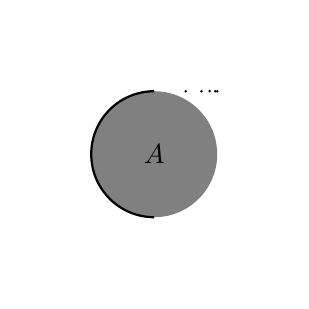
\begin{tikzpicture}[x=0.8cm,y=0.8cm]
    \draw[white] (2,-2) -- (2,2) -- (-2,2) -- (-2,-2) -- (2,-2);
    \fill[black!50] (0,0) circle (1);
    \draw[thick] (0,1) arc (90:270:1);
    \foreach \x in {0.5,0.75,0.88,0.97,1.0}
      \fill (\x,1) circle (0.5pt);
    \draw (0,0) node {$A$};
  \end{tikzpicture}
  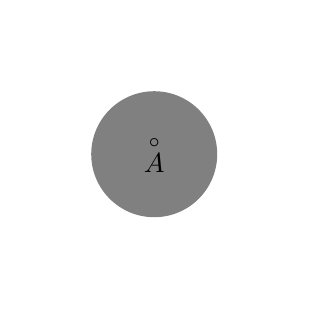
\begin{tikzpicture}[x=0.8cm,y=0.8cm]
    \draw[white] (2,-2) -- (2,2) -- (-2,2) -- (-2,-2) -- (2,-2);
    \fill[black!50] (0,0) circle (1);
    \draw (0,0) node {$\stackrel \circ A$};
  \end{tikzpicture}
  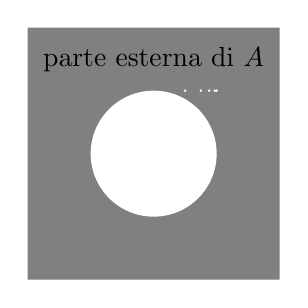
\begin{tikzpicture}[x=0.8cm,y=0.8cm]
    \fill[black!50] (2,-2) -- (2,2) -- (-2,2) -- (-2,-2) -- (2,-2);
    \foreach \x in {0.5,0.75,0.88,0.97,1.0}
      \fill[white] (\x,1) circle (0.5pt);
    \fill[white] (0,0) circle (1);
    \draw (0,1.5) node {parte esterna di $A$};
  \end{tikzpicture}
  \begin{tikzpicture}[x=0.8cm,y=0.8cm]
    \draw[white] (2,-2) -- (2,2) -- (-2,2) -- (-2,-2) -- (2,-2);
    \foreach \x in {0.5,0.75,0.88,0.97,1.0}
      \fill (\x,1) circle (0.5pt);
    \draw[thick] (1,0) arc (0:360:1);
    \draw (0,0) node {$\partial A$};
  \end{tikzpicture}
  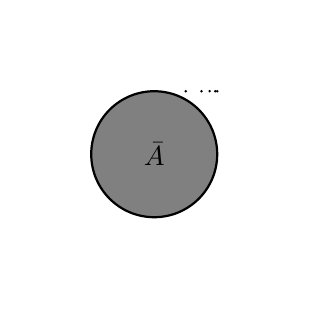
\begin{tikzpicture}[x=0.8cm,y=0.8cm]
    \draw[white] (2,-2) -- (2,2) -- (-2,2) -- (-2,-2) -- (2,-2);
    \foreach \x in {0.5,0.75,0.88,0.97,1.0}
      \fill (\x,1) circle (0.5pt);
    \fill[black!50] (0,0) circle (1);
    \draw[thick] (1,0) arc (0:360:1);
    \draw (0,0) node {$\bar A$};
  \end{tikzpicture}
  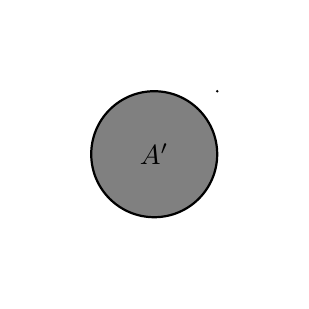
\begin{tikzpicture}[x=0.8cm,y=0.8cm]
    \draw[white] (2,-2) -- (2,2) -- (-2,2) -- (-2,-2) -- (2,-2);
    \fill (1,1) circle (0.5pt);
    \fill[black!50] (0,0) circle (1);
    \draw[thick] (1,0) arc (0:360:1);
    \draw (0,0) node {$A'$};
  \end{tikzpicture}
\caption{Un insieme $A$
e la sua parte interna $\stackrel \circ A$,
parte esterna, frontiera $\partial A$, chiusura $\bar A$ e punti di
accumulazione $A'$.}
\label{fig:}
\end{figure}


\begin{definition}[relazioni e proprietà topologiche]
\mymark{*}
\label{def:466342}
Sia $(X,d)$ uno spazio metrico.
Un insieme $A\subset X$ si dirà essere un insieme
\myemph{aperto} in $X$ se per ogni $x\in A$ esiste $r>0$
tale che $B_r(x) \subset A$.
Un insieme $A\subset X$ si dirà essere un insieme \myemph{chiuso} in $X$ se il suo complementare $X\setminus A$ è aperto.

La famiglia di tutti gli insiemi aperti si chiama \myemph{topologia} dello spazio metrico $X$. Tutte le definizioni che seguono non dipendono dalla distanza $d$ ma solamente dalla topologia: basterà usare aperti qualunque al posto delle palle $B_r(x)$.

Se $A\subset X$ è un insieme qualunque
$x\in X$ è un punto qualunque diremo che:
\begin{enumerate}
\item
$x$ è \myemph{punto!interno} ad $A$ se esiste $r>0$ tale che $B_r(x) \subset A$;
chiameremo
\myemph{parte!interna}
di $A$ l'insieme dei punti interni di $A$
e la denoteremo con $\stackrel\circ A$;
\item
$A$ è un \myemph{intorno} di $x$ se $x$ è punto interno ad $A$
ovvero esiste $r>0$ tale che $B_r(x)\subset A$;
\item
$x$ è \myemph{punto!esterno} ad $A$ se è interno al complementare di $A$ ovvero esiste $r>0$ tale che $B_r(x) \cap A = \emptyset$;
chiameremo \myemph{parte!esterna} di $A$ l'insieme dei punti esterni ad $A$;
\item
$x$ è \myemph{punto!di frontiera} per $A$ se non è né interno né esterno ad $A$ ovvero per ogni $r>0$ l'insieme $B_r(x)$ contiene punti di $A$ e di $X\setminus A$;
chiameremo \myemph{frontiera} (o bordo) di $A$ l'insieme dei punti di frontiera che denoteremo con $\partial A$.
\item
$x$ è \myemph{punto!di aderenza} di $A$ se è interno o di frontiera ovvero se per ogni $r>0$ si ha $B_r(x) \cap A \neq \emptyset$;
chiameremo \emph{chiusura} di $A$ l'insieme dei punti di aderenza,
che denoteremo con $\bar A$;
\mymargin{chiusura}
\index{chiusura}
\item
$x$ è \myemph{punto!di accumulazione} di $A$ se
è punto di aderenza per $A \setminus \ENCLOSE{x}$ ovvero se
per ogni $r>0$ l'insieme $A \cap B_r(x)$ contiene punti diversi da $x$, chiameremo \myemph{derivato} di $A$ l'insieme dei punti di accumulazione (che si potrebbe denotare con $A'$);
\item
$x$ è \myemph{punto!isolato} di $A$ se è un punto di $A$ ma non di accumulazione per $A$ cioè se esiste $r>0$ per cui
$B_r(x) \cap A = \ENCLOSE{x}$.
\end{enumerate}
\end{definition}

\begin{theorem}[le palle sono aperte]
Sia $(X,d)$ uno spazio metrico, sia $x\in X$ e $r>0$. Allora la palla $B_r(x)$ è un insieme aperto in $X$.
\end{theorem}
%
\begin{proof}
Sia $y\in B_r(x)$: è sufficiente trovare $\rho>0$ tale che $B_\rho(y) \subset B_r(x)$. Prendendo $\rho = r-d(y,x)$ si osserva che $\rho >0 $ e, per la disuguaglianza triangolare,
dato $z \in B_\rho(y)$ si ha
\[
  d(z,x) \le d(z,y) + d(y,x) < \rho + d(y,x) = r
\]
da cui $B_\rho(y)\subset B_r(x)$ come volevamo dimostrare.
\end{proof}

\begin{comment}
\section{spazi topologici}

\begin{definition}[spazio topologico]
Sia $X$ un insieme e sia $\tau\subset \P(X)$ una famiglia di sottoinsiemi di $X$.
Diremo che $X$ è uno \myemph{spazio topologico}, che $\tau$ è una
\myemph{topologia} e che gli elementi di $\tau$ sono \myemph{aperti}
se:
\begin{enumerate}
\item $\emptyset \in \tau$, $X\in \tau$ (il vuoto e l'intero spazio sono aperti);
\item $A \subset \tau \implies \bigcup A \in \tau$ (unione qualunque di aperti è aperta);
\item $A,B\in \tau \implies A \cap B \in \tau$ (intersezione finita di aperti è aperta).
\end{enumerate}
Diremo inoltre che lo spazio topologico è \myemph{separato} (o $T_2$ o di Hausdorff)
\index{spazio topologico!separato}
\index{spazio topologico!$T_2$}
\index{spazio topologico!di Hausdorff}
\index{$T_2$}
\index{separato}
se inoltre vale
\begin{enumerate}
\item[4.] dati $x,y\in X$ con $x\neq y$ esistono $U,V\in \tau$ con $x\in U$,
$y\in V$ e $U\cap V=\emptyset$.
\end{enumerate}

Diremo che un sottoinsieme $A\subset X$ è \myemph{chiuso} se il complementare
è aperto ($X\setminus A\in \tau$).
Diremo che $A\subset X$ è un \myemph{intorno} del punto $a\in X$ se esiste $U\in \tau$
tale che $x\in U \subset A$.

Tutte le proprietà date nella definizione~\ref{def:466342} possono quindi essere
date in uno spazio topologico utilizzando gli intorni (o gli aperti) al posto
delle palle.
\end{definition}

\begin{theorem}[topologia indotta dalla metrica]
Sia $X$ uno spazio metrico e sia $\tau$ l'insieme di tutti gli aperti
di $X$ ovvero:
\[
 \tau = \ENCLOSE{A \subset X\colon \forall a \in A \exists \rho>0 \colon B_\rho(a)\subset A}.
\]
Allora $\tau$ è una topologia e $X$ è uno spazio topologico separato rispetto alla topologia
$\tau$.
\end{theorem}

\begin{definition}[base di intorni]
Sia $X$ un insieme e per ogni $x\in X$ sia data $\B_x\subset \P(X)$
una famiglia di sottoinsiemi di $X$. Diremo che $\B_x$ è una
\myemph{base di intorni} di $x$ se valgono le seguenti proprietà:
\begin{enumerate}
\item $\B_x$ è non vuoto;
\item se $B\in \B_x$ allora $x \in B$;
\item se $A,B\in \B_x$ allora esiste $C\in \B_x$ tale che $C\subset A\cap B$;

\item Se un insieme contiene un intorno di un punto anch'esso è un intorno di quel punto.
\item L'intersezione di due intorni di un punto è un intorno del punto.
\end{enumerate}

Se per ogni $x\in X$ l'insieme $\B_x$ è una base di intorni di $x$ potremo
definire
\[
  \tau = \ENCLOSE{A \subset X\colon \forall x\in A \exists B \in \B_x \colon B\subset A}
\]
e risulta che $\tau$ è una topologia e quindi $X$ è uno spazio topologico
rispetto a tale topologia (indotta dalla base di intorni).

Se inoltre vale anche la seguente proprietà:
\begin{enumerate}
\item dati $x,y\in X$, $x\neq y$, esistono $B\in \B_x$ e $C\in \B_y$ tali che
$B\cap C=\emptyset$;
\end{enumerate}
allora $X$ sarà uno spazio topologico separato.
\end{definition}
%


Le proprietà seguenti sono conseguenza degli assiomi precedenti e sono quindi valide in ogni spazio topologico.

\begin{enumerate}
\item
La parte interna di un qualunque $A\subset X$ è il più grande (ovvero l'unione di ogni) aperto contenuto in $A$. La chiusura di $A$ è il più piccolo (ovvero l'intersezione di ogni) chiuso contenente $A$.
In particolare la parte interna è sempre aperta e la parte interna di un aperto è tutto l'insieme. La chiusura è un insieme chiuso e la chiusura di un chiuso è l'insieme stesso.
\item
La frontiera di un insieme è chiusa. Parte interna, frontiera e parte esterna sono tre insiemi disgiunti (rispettivamente aperto, chiuso e aperto) la cui unione è tutto lo spazio.
\end{enumerate}

\begin{theorem}
Se $X$ è uno spazio metrico la famiglia di insiemi
\[
  \tau = \ENCLOSE{A \subset X \colon \forall a \in A \exists \rho>0 \colon B_\rho(x) \subset A}
\]
risulta essere una topologia su $X$ che si chiama \emph{topologia indotta}
dalla metrica di $X$.
\end{theorem}
%
\begin{proof}
L'insieme vuoto è aperto in quanto non ci sono punti su cui è necessario verificare la proprietà che definisce gli aperti. Anche l'intero spazio è aperto in quanto ogni palla è contenuta in esso. Dunque $\emptyset, X$ sono aperti e di conseguenzi i rispettivi complementari: $X, \emptyset$ sono chiusi.

Che l'unione qualunque di aperti sia aperta è ovvio: preso un punto dell'unione tale punto è contenuto in uno degli aperti. Dunque c'è una palletta centrata nel punto e contenuta nell'aperto. Ma allora essa è anche contenuta nell'unione.
Che l'intersezione di chiusi sia un chiuso si ottiene passando ai complementari: il complementare di un chiuso è un aperto e il complementare dell'intersezione è l'unione dei complementari.

L'intersezione qualunque di chiusi è uguale al complementare (rispetto ad $X$) dell'unione dei complementari. Per definizione il complementare di un chiuso è aperta e dunque l'unione dei complementari è aperta. Dunque il suo complementare è un chiuso.

Consideriamo ora l'intersezione $A\cap B$ di due aperti $A$ e $B$. Se $x$ è un punto dell'intersezione sappiamo che esistono due palle $B_r(x)$ e $B_s(x)$ tali che $B_r(x)\subset A$ e $B_s(x) \subset B$. La più piccola delle due è contenuta in $A\cap B$ e questo dimostra che $A\cap B$ è aperto. Passando ai complementari si ottiene che l'unione di due chiusi è un chiuso.

Dati $x,y \in X$ se $x\neq y$ allora $r=d(x,y)/2>0$. Osserviamo allora che $B_r(x)$ e $B_r(y)$ sono disgiunte in quanto se se esistesse $z\in B_r(x) \cap B_r(y)$ si avrebbe $d(x,y)\le d(x,z) + d(z,y) < r + r = d(x,y)$ che è assurdo.

Abbiamo quindi dimostrato le quattro proprietà degli aperti. Passiamo alle proprietà degli intorni. Per definizione un insieme $U$ è un intorno di $x$ se esiste un aperto $A$ tale che $x\in A \subset U$. Necessariamente quindi $x\in U$. E se $V\supset U$ allora $x\in A \subset V$ e dunque anche $V$ è intorno di $x$. Se $U$ e $V$ sono intorni dovranno esistere due aperti $A$ e $B$ tali che $x\in A \subset U$ e $x \in B \subset V$. Ma allora $A\cap B$ è aperto e $x \in A \cap B \subset U \cap V$ dunque $U\cap V$ è anch'esso un intorno di $x$. Per il quarto punto basta osservare che ogni intorno contiene, per definizione, un aperto che contiene il punto e un aperto è, sempre per definizione, intorno di ogni suo punto. Per il punto 5 già sappiamo che due punti distinti sono contenuti in aperti disgiunti, e gli aperti sono sempre intorni di ogni loro punto.

Dimostriamo ora che la parte interna di un insieme $A$ è l'unione di tutti gli aperti contenuti in $A$. Da un lato se $x$ è un punto interno ad $A$ allora esiste $r>0$ tale che $B_r(x)\subset A$. Essendo $B_r(x)$ aperto risulta quindi che $x$ sta nell'unione degli aperti contenuti in $A$. Viceversa se $x$ sta nell'unione di tutti gli aperti contenuti in $A$ deve esistere un aperto $U$ tale che $x\in U \subset A$. Ma allora esiste $r>0$ tale che $B_r(x) \subset U \subset A$ e dunque $x$ è punto interno ad $A$. La proprietà analoga per i chiusi si ottiene passando ai complementari.

La frontiera di un insieme è, per definizione, l'insieme dei punti che non sono né interni né esterni. D'altra parte è chiaro che un punto non può essere contemporaneamente interno ed esterno. Dunque la frontiera è il complementare dell'unione della parte interna e della parte esterna, ed è quindi un insieme chiuso.
\end{proof}
\end{comment}

\begin{theorem}[chiusura sequenziale]
Sia $(X,d)$ uno spazio metrico.
Un insieme $A\subset X$ è chiuso se e solo se
per ogni successione $a_n\in A$ se $a_n\to a\in X$ allora $a \in A$
(il limite di punti di $A$, se esiste, è un punto di $A$).
\end{theorem}
%
\begin{proof}
Supponiamo che $A$ sia chiuso e sia
$a_k \in A$ una successione convergente ad un punto di $X$: $a_k \to a$.
Dobbiamo mostrare che $a\in A$.
Per definizione di convergenza
sappiamo che per ogni $\eps>0$ esiste $K\in \NN$ tale per ogni $k> K$
si ha $d(a_k,a)<\eps$ e quindi $a_k \in B_\eps(a)$.
In particolare $A \cap B_\eps(a) \neq \emptyset$.
Risulta quindi che $a$ non è esterno ad $A$ e quindi, essendo $A$ chiuso, $a\in A$.

Supponiamo che $A$ non sia chiuso e verifichiamo che in tal caso
si può trovare una successione $a_k$ di punti di $A$ che converge $a_k\to a$
ad un punto $a\not\in A$.
Se $A$ non è chiuso significa che c'è un punto $a \in X\setminus A$ che non è esterno ad $A$.
Ciò vuol dire che per ogni $r>0$ l'insieme $B_r(y)\cap A$ è non vuoto. Per ogni $k\in \NN$ posso allora
scegliere $r=1/k$ e quindi so che esiste un punto $a_k\in B_r(a) \cap A$ ovvero $a_k \in A$ e
$d(a_k,a) < 1/k$.
Dunque $a_k \to a$ con $a_k\in A$ ma $a\not \in A$, come volevamo dimostrare.
\end{proof}

\begin{definition}[continuità]
\mymark{**}
Una funzione $f\colon X \to Y$ definita tra due spazi metrici
si dice essere \myemph{sequenzialmente!continua} nel punto $x\in X$ se
per ogni successione convergente $x_n \to x$ in $X$ 
risulta che $f(x_n)\to f(x)$ in $Y$.
Diremo che $f$ è \emph{sequenzialmente continua} se è sequenzialmente continua
in ogni punto $x$ del suo dominio $X$.

Una funzione $f\colon X \to Y$ definita tra due spazi metrici
si dice essere \myemph{continua} in un punto $x\in X$ se
\begin{equation}\label{eq:continuita_metrico}
 \forall \eps>0\colon \exists \delta>0\colon \forall y \in X \colon
 d(x,y)< \delta \implies d(f(x), f(y)) < \eps.
\end{equation}
Diremo che $f$ è \emph{continua} se
è continua in ogni punto $x$ del suo dominio.
\end{definition}

Anche in questo caso abbiamo considerato due diverse nozioni di continuità che
in generale (in spazi topologici) potrebbero non coincidere ma nel caso degli
spazi metrici sono equivalenti, come dimostriamo nel seguente teorema.

\begin{theorem}[definizioni equivalenti di continuità]
Sia $f\colon X \to Y$ una funzione definita tra due spazi metrici $X$ e $Y$.
Allora $f$ è sequenzialmente continua in un punto $x\in X$ se e solo se è
continua nel punto $x$.

Inoltre $f$ è continua se e solo se
per ogni $A$ aperto in $Y$ risulta che $f^{-1}(A)$ è aperto in $X$
(la controimmagine di un aperto è aperta).
\end{theorem}
%
\begin{proof}
Supponiamo che $f$ sia sequenzialmente continua in $x$
e, per assurdo, supponiamo che $f$ non sia continua nello stesso punto $x$.
Allora negando~\eqref{eq:continuita_metrico} otteniamo che esiste $\eps>0$
tale che per ogni $\delta>0$ in particolare per ogni $\delta = \frac{1}{k}$
con $k\in \NN$ esiste un punto $y_k$ tale che $d(y_k,x)<\frac 1 k$ ma
$d(f(y_k),f(x))\ge \eps$. Significa che $y_k \to x$ e quindi,
se $f$ è sequenzialmente continua, dovrebbe essere $f(y_k)\to f(x)$. Ma
questo è in contraddizione con la condizione $d(f(y_k),f(x))\ge \eps$.

Viceversa supponiamo che $f$ sia continua in $x$ e consideriamo una qualunque
successione $x_k \to x$.
Per dimostrare che $f(x_k)\to f(x)$ dobbiamo verificare che per ogni
$\eps>0$ esiste $K\in \NN$ tale che per ogni $k>K$ si ha $d(f(x_k),f(x)) < \eps$.
Ma dalla continuità di $f$, dato $\eps>0$ sappiamo esistere $\delta>0$ per cui
se $d(y,x)<\delta$ allora $d(f(y),f(x))<\eps$. Visto che $x_k\to x$
certamente esiste $K\in \NN$ tale che per ogni $k>K$ si ha $\abs{x_k-x}<\delta$
e quindi $\abs{f(x_k)-f(x)}< \eps$ come volevamo dimostrare.

Mostriamo ora che se $f$ è continua e $A$ è aperto in $Y$ allora $f^{-1}(A)$
è aperto in $X$.
Dato un punto qualunque $x_0\in f^{-1}(A)$ sappiamo che $f(x_0)\in A$ dunque, essendo
$A$ aperto, esiste $\eps>0$ tale che $B_\eps(f(x_0))\subset A$.
Per la continuità di $f$ esiste allora $\delta>0$ tale che se $\abs{x-x_0} < \delta$
allora $\abs{f(x)-f(x_0)}<\eps$ e quindi $f(x)\in A$. Significa che $B_\delta(x_0)\subset f^{-1}(A)$.
Questo è vero per ogni $x_0\in f^{-1}(A)$ quindi tale insieme è aperto.

Viceversa supponiamo che la controimmagine di ogni aperto sia un aperto e
dimostriamo che la funzione è continua in ogni punto.
Preso un punto $x_0\in X$ e un $\eps>0$ consideriamo l'aperto $B_\eps(f(x_0))$.
La sua controimmagine è l'insieme $\ENCLOSE{x\colon \abs{f(x)-f(x_0)} < \eps}$ e
per ipotesi sappiamo che è aperto. Significa allora che esiste $\delta>0$
tale $B_\delta(x_0)$ è contenuto in tale insieme, ovvero per ogni $x\in B_\delta(x_0)$
cioè $\abs{x-x_0}<\delta$
risulta $f(x) \in B_\eps(f(x_0))$
cioè $\abs{f(x)-f(x_0)}<\eps$.
Abbiamo quindi verificato la definizione di
continuità nel punto $x_0$.
\end{proof}

\begin{definition}[spazi limitati]
\mymark{*}
Sia $X$ uno spazio metrico o un sottoinsieme di uno sottospazio metrico. Si dirà che $X$ è
\myemph{limitato} se è contenuto in una palla ovvero se
esiste $x_0\in X$ e $R>0$ tale che $X\subset B_R(x_0)$.
\end{definition}

\begin{definition}[compattezza sequenziale]
\mymark{**}
Sia $X$ uno spazio metrico o un sottoinsieme di uno
spazio metrico. Si dirà che $X$ è
\myemph{sequenzialmente!compatto} se da ogni
successione $x_k \in X$ è possibile estrarre una sottosuccessione $x_{k_j}\to x$
convergente ad un punto $x\in X$.
\end{definition}

La definizione più generale di compattezza viene data negli spazi topologici.
Nel contesto generale compattezza e compattezza sequenziale sono concetti
diversi ma nell'ambito degli spazi metrici i due concetti coincidono.
Per questo potremo scrivere più brevemente \myemph{compatto}
al posto di \emph{sequenzialmente compatto} quando lavoriamo negli spazi metrici.

Il teorema di Bolzano-Weierstrass afferma che gli intervalli $[a,b]$ con
$a,b\in \RR$ sono compatti.
Più in generale si può dimostrare che tutti gli insiemi chiusi e limitati
di $\RR^n$ sono compatti. In generale questo risultato non è vero in qualunque
spazio metrico (un esempio negativo è dato dalla convergenza uniforme, come
vedremo più avanti) ma l'implicazione inversa è sempre vera, come enunciato nel
seguente teorema.

\begin{theorem}
\mymark{**}
Se $A$ è un sottoinsieme sequenzialmente
compatto di uno spazio metrico $X$
allora $A$ è chiuso e limitato.
\end{theorem}
%
\begin{proof}
Chiaramente $A$ è chiuso in quanto presa una successione $x_k\in A$ convergente a punto $x\in X$
sappiamo che esiste una sottosuccessione convergente ad un punto di $A$. Ma necessariamente ogni sottosuccessione converge ad $x$ quindi $x\in A$. Se $A$ non fosse limitato
fissato $a\in A$ per ogni $k\in \NN$ dovrebbe esistere un punto $x_k\in A$ tale che $x_k \not\in B_k(a)$
cioè $d(x_k,a) > k$. Supponiamo allora che esista una sottosuccessione convergente $x_{k_j}\to x \in A$. Allora per la disuguaglianza triangolare inversa si avrebbe
\[
  d(x, a) \ge d(x_{k_j}, a) - d(x_{k_j},x)
   \ge k_j - d(x_{k_j},x) \to +\infty - 0 = +\infty.
\]
Ma questo è assurdo in quanto $d(x,a)\in \RR$.
\end{proof}

\begin{theorem}[Weierstrass: le funzioni continue mandano compatti in compatti]
Sia $f\colon X \to Y$ una funzione continua tra
due spazi metrici $X$ e $Y$.
Se $K\subset X$ è sequenzialmente compatto allora
anche $f(K)$ è sequenzialmente compatto.
\end{theorem}
%
\begin{proof}
Sia $y_k \in f(K)$ una qualunque successione. Allora
esiste $x_k \in K$ tale che $f(x_k) = y_k$.
Essendo $K$ compatto possiamo estrarre una sottosuccessione convergente: $x_{k_j}\to x$. Essendo $f$ continua si ha
\[
  y_{k_j} = f(x_{k_j}) \to f(x) \in f(K).
\]
\end{proof}

Nel caso $X=Y=\RR$ recuperiamo l'usuale teorema di Weierstrass, in quanto se $f\colon [a,b]\to \RR$ è continua essendo $[a,b]$ compatto risulta che $f([a,b])$ è compatto. Ma i compatti di $\RR$ sono chiusi e limitati quindi hanno massimo e minimo in quanto l'estremo superiore e l'estremo inferiore sono finiti e sono punti di aderenza dell'insieme.

\begin{definition}[uniforme continuità]
  Sia $f\colon X \to Y$ una funzione definita tra due spazi metrici $X$ e $Y$.
  Diremo che $f$ è \myemph{uniformemente continua} se 
  \[
  \forall \eps>0 \colon \exists \delta>0 \colon 
    d(x,x')< \delta \implies d(f(x),f(x'))<\eps. 
  \]
\end{definition}

\begin{theorem}[Heine-Cantor]
  \mymargin{Heine-Cantor}%
  \index{teorema!di Heine-Cantor}%
Sia $X$ uno spazio metrico sequenzialmente compatto e $Y$ uno spazio metrico.
Sia $f\colon X\to Y$ una funzione continua. Allora $f$ è uniformemente continua.
\end{theorem}
%
\begin{proof}
  La dimostrazione è identica a quella già fatta nel corrispondente 
  teorema~\ref{th:heine_cantor} per le funzioni di variabile reale.
\end{proof}

\section{completezza}

\begin{definition}[successioni di Cauchy]
\mymark{***}
\index{successione!di Cauchy}
\index{Cauchy!successione di}
Sia $(X,d)$ uno spazio metrico e $x_k$ una successione di punti di $X$.
Diremo che $x_k$ è una
\emph{successione di Cauchy}
\mynote{successione di Cauchy}
se
\[
 \forall \eps>0\colon \exists n\in \NN\colon \forall j>n \colon \forall k > n \colon d(x_j,x_k) < \eps.
\]
\end{definition}

La proprietà che definisce le successioni di Cauchy
si potrebbe anche scrivere così:
\[
  \lim_{k \to +\infty} \sup_{j\ge k} d(x_j, x_k) = 0.
\]

\begin{theorem}[le successioni convergenti sono di Cauchy]
\mymark{**}%
\label{th:se_converge_cauchy}
Sia $x_k\to x$ una successione convergente in uno spazio metrico $(X,d)$. Allora $x_k$ è di Cauchy.
\end{theorem}
%
\begin{proof}
\mymark{**}
Per definizione se $x_k \to x$ si ha
\[
  \forall \eps>0\colon \exists n\in \NN \colon
  \forall k>n \colon d(x_k,x)< \eps.
\]
Applicando la disuguaglianza triangolare, per ogni $j,k>n$
si ottiene il risultato desiderato:
\[
  d(x_j, x_k) \le d(x_k,x) + d(x,x_j) \le 2\eps.
\]
\end{proof}

\begin{definition}[completezza]
\mymark{***}
\mynote{completezza}
\index{completezza}
Uno spazio metrico $(X,d)$ si dice essere \myemph{completo}
se ogni successione di Cauchy è convergente.
\end{definition}

Il prototipo di spazio metrico completo è $\RR$, come vedremo nel teorema~\ref{th:R-completo}.
Un esempio di spazio metrico non completo è $\QQ$.
Infatti se prendiamo una
successione $q_n \in\QQ$ con $q_n\to \sqrt 2$ la successione $q_n$ è convergente
in $\RR$ e quindi è di Cauchy in $\RR$. Ma visto che $q_n\in \QQ$ risulta
che $q_n$ è di Cauchy anche in $\QQ$ (la condizione di Cauchy è la stessa).
Ma in $\QQ$ tale successione non converge in quanto $\sqrt 2\not \in \QQ$.

\begin{definition}[spazio di Banach]
Uno spazio vettoriale normato si dice essere uno
\emph{spazio di Banach}%
\mynote{spazio di Banach}%
\index{spazio!di Banach}%
\index{Banach!spazio di}
se, come spazio metrico, risulta essere completo.
Se la norma è euclidea, cioè deriva da un prodotto scalare, lo spazio si dirà
\emph{spazio di Hilbert}.
\mynote{spazio di Hilbert}%
\index{spazio!di Hilbert}
\end{definition}

\begin{lemma}
\label{lm:cauchy_limitata}
Ogni successione di Cauchy è limitata
(più precisamente: se $x_n$ è una successione di Cauchy in uno spazio metrico $X$ allora l'insieme $\ENCLOSE{x_n\colon n\in \NN}$
è un insieme limitato).
\end{lemma}
%
\begin{proof}
Sia $x_k \in \RR$ una successione di Cauchy.
Fissato $\eps =1$ sappiamo che esiste $N\in \NN$
per cui per ogni $k,j>N$ si ha
$d(x_k,x_j) < 1$. In particolare per ogni $k>N$ si ha
\[
  d(x_k, x_{N+1}) < 1.
\]
Dunque posto
\[
  R = \max\ENCLOSE{d(x_0,x_1), d(x_0,x_2), \dots, d(x_0,x_N), d(x_0, x_{N+1}) + 1}
\]
si osserva che per ogni $k\in \NN$ si ha $d(x_0, x_k)\le R < R+1$ in quanto 
se $k \le N$ abbiamo scelto appositamente $R$ in modo che sia più grande di $d(x_0,x_k)$ e se $k > N$ allora
\[
  d(x_0,x_k) \le d(x_0,x_{N+1}) + d(x_{N+1},x_k)
    \le d(x_0,x_{N+1}) + 1 \le R.
\]

Significa quindi che per ogni $x\in \NN$ si ha $x_k \in B_{R+1}(x_0)$ che è la definizione di limitatezza in uno
spazio metrico.
\end{proof}

\begin{lemma}
\label{lm:cauchy_estratta_convergente}
Se una successione di Cauchy ha una sottosuccessione convergente, allora l'intera successione è convergente.
\end{lemma}
%
\begin{proof}
Sia $x_k$ la successione di Cauchy e sia $x_{k_j}\to x$ una  sottosuccessione convergente.
Allora per ogni $\eps>0$
esiste $m$ tale che se $k,j>m$ allora $d(x_k ,x_j) < \eps$.
Visto che $x_{k_j} \to x$ possiamo trovare $j$ tale che $k_j > m$ e tale che $d(x_{k_j},x) < \eps$. Ma allora
\[
  d(x_k,x) \le d(x_k, x_{k_j}) + d(x_{k_j},x)
   \le 2 \eps.
\]
E questo è vero per ogni $k > m$ da cui risulta verificata la definizione di limite $x_k \to x$.
\end{proof}

\begin{theorem}[completezza di $\RR$]
\mymark{***}%
\mynote{$\RR$ è completo}%
\index{completezza!di $\RR$}%
\label{th:R-completo}%
$\RR$ è completo.
\end{theorem}
%
\begin{proof}
\mymark{***}
Dobbiamo dimostrare che se $x_k$ è una successione di Cauchy in $\RR$ allora $x_k$ converge.
Per il lemma~\ref{lm:cauchy_limitata} sappiamo che $x_k$ è limitata.
Ma allora per il teorema di Bolzano-Weierstrass sappiamo che $x_k$ ha
una estratta convergente.
Grazie al lemma~\ref{lm:cauchy_estratta_convergente} possiamo quindi concludere
che la successione $x_k$ è essa stessa convergente.
\end{proof}

\begin{corollary}[completezza di $\RR^n$ e $\CC$]
Gli spazi $\RR^n$ e $\CC$ (con la usuale distanza euclidea)
sono completi.
\end{corollary}
%
\begin{proof}
Basta osservare che la convergenza (o la condizione di Cauchy) di una successione in $\RR^n$ si ha se e solo se ogni componente è convergente (o di Cauchy) in $\RR$. Dunque essendo $\RR$ completo anche $\RR^n$ lo è. Come spazio metrico $\CC$ è isomorfo ad $\RR^2$ dunque anch'esso è completo.
\end{proof}

\begin{theorem}[completezza dei compatti]
Ogni spazio metrico compatto è completo.
\end{theorem}
%
\begin{proof}
Visto che lo spazio è compatto ogni successione di Cauchy
ammette una sottosuccessione convergente.
Ma allora, grazie al lemma~\ref{lm:cauchy_estratta_convergente},
l'intera successione converge e dunque lo spazio è completo.
\end{proof}

\begin{theorem}[chiusi in spazi compatti e in spazi completi]
Sia $(X,d)$ uno spazio metrico e sia $A\subset X$ un sottoinsieme chiuso in $X$. Se $X$ è compatto allora anche $A$ è compatto, se $X$ è completo allora anche $A$ è completo.
\end{theorem}
\begin{proof}
Se $X$ è compatto da ogni successione in $A$ si può estrarre una sottosuccessione convergente ad un punto di $X$. 
Ma siccome $A$ è chiuso il punto sta in $A$ e dunque la sottosuccessione è convergente in $A$.

Una successione di Cauchy in $A$ è di Cauchy anche in $X$. 
Se $X$ è completo tale successione converge ad un punto di $X$. 
Se $A$ è chiuso tale punto è in $A$ e dunque la successione converge in $A$.
\end{proof}

\begin{theorem}[estendibilità delle funzioni uniformemente continue]
\mymark{**}%
\label{th:estensione_uniformemente_continua}%
Sia $f\colon A \subset X \to Y$ una funzione definita su un sottoinsieme $A$
di uno spazio metrico $X$ a valori in uno spazio metrico completo $Y$
(ad esempio $X=\RR$ e $Y=\RR$). Se $f$ è uniformemente continua allora
esiste una unica funzione continua $\tilde f \colon \bar A \to Y$
tale che per ogni $x\in A$ si ha $\tilde f(x) = f(x)$.
Inoltre $\tilde f$ è anch'essa uniformemente continua.
\end{theorem}
%
\begin{proof}
La prima osservazione è
che se una funzione $f$ è uniformemente continua allora $f$
manda successioni di Cauchy in successioni di Cauchy.
Infatti se $f$ è uniformemente continua si ha
\[
 \forall \eps>0\colon \exists \delta>0 \colon d(x,y)<\delta \implies d(f(x),f(y))<\eps
\]
e se $a_n$ è di Cauchy si ha
\[
 \exists N\in\NN \colon k,j>N \implies d(a_k,a_j)< \delta
\]
dunque mettendo insieme le due proprietà
si ottiene la condizione
di Cauchy per $f(a_k)$:
\[
\forall \eps>0\colon \exists N\in \NN\colon k,j>N \implies d(f(a_k),f(a_j))< \eps.
\]

Preso un punto $x \in \bar A$ esiste certamente $a_n \in A$ con $a_n\to x$.
Vogliamo dimostrare che $f(a_n)$ ha limite in $Y$ e che tale limite non
dipende dalla successione $a_n$ scelta. Se $a_n \to a$ allora $a_n$ è di Cauchy in $X$
(teorema~\ref{th:se_converge_cauchy}).
Per quanto detto prima possiamo affermare che anche $f(a_n)$ è di Cauchy
e quindi converge in $Y$, in quanto $Y$ è completo per ipotesi.
Inoltre il $\lim f(a_n)$ non dipende dalla successione scelta perché
se $b_n\to x$ fosse un'altra successione potremmo costruire una successione
$c_n$ che alterna i punti di $a_n$ e $b_n$ (ponendo, ad esempio, $c_{2n} = a_n$ e
$c_{2n+1} = b_n$). Anche $c_n \to x$ ed è di Cauchy, dunque $f(c_n)$ converge.
Ma $f(a_n)$ e $f(b_n)$ sono sotto-successioni di $f(c_n)$ e dunque convergono
allo stesso limite.
Abbiamo quindi dimostrato che per ogni $x\in \bar A$ esiste $\ell \in Y$
tale che se $a_n\to x$, $a_n\in A$ allora $f(a_n) \to \ell$. Possiamo
quindi definire $\tilde f(x)=\ell$. Se esiste una estensione continua di
$f$ non può che essere definita in questo modo, in quanto le funzioni continue
mandano successioni convergenti in successioni convergenti.

D'altra parte possiamo dimostrare che $\tilde f$ è una funzione uniformemente continua.
Infatti per ogni $\eps>0$ possiamo scegliere $\delta>0$ dato dall'uniforme
continuità di $f$: dati $x,y\in \bar A$ con $d(x,y)<\delta/3$ esisteranno
$x_n,y_n \in A$ con $x_n\to x$, $y_n\to y$. Si potrà quindi trovare $n$
sufficientemente grande in modo che
$d(x_n,x)<\delta/3$, $d(y_n,y)<\delta/3$,
$d(f(x_n),\tilde f(x)) < \eps$, $d(f(y_n),\tilde f(y)) < \eps$.
Si avrà allora
$d(x_n,y_n)< d(x_n,x)+d(x,y)+d(y,y_n) < \delta$, dunque $d(f(x_n),f(y_n))<\eps$
e in conclusione
\[
d(f(x),f(y))
\le d(f(x),f(x_n)) + d(f(x_n),f(y_n)) + d(f(y_n),f(y))
\le 3\eps.
\]
Abbiamo quindi dimostrato l'uniforme continuità di $\tilde f$ con $3\eps$ al posto
di $\eps$ e $\delta/3$
al posto di $\delta$.
\end{proof}

\begin{definition}[lipschitz]
\mymark{***}
Sia $f\colon X \to Y$ una funzione definita tra due spazi metrici e sia $L\ge 0$.
Dato $L\ge 0$
diremo che $f$ è $L$-lipschitziana se
\index{funzione!lipschitziana}
per ogni $x,y \in X$ si ha
\[
  d(f(x),f(y)) \le L \cdot d(x,y).
\]
Diremo che $f$ è lipschitziana se esiste $L\ge 0$ tale che $f$ sia $L$-lipschitziana.
\end{definition}

\begin{theorem}
\label{th:lipschitz_uniformemente_continua}%
\mymark{*}%
Se $f\colon X \to Y$ è lipschitziana allora
$f$ è sequenzialmente continua, cioè
\[
  x_k \to x \implies f(x_k)\to f(x).
\]
\end{theorem}
%
\begin{proof}
Se $x_k\to x$ significa che $d(x_k,x) \to 0$, quindi
\[
  d(f(x_k), f(x)) \le L \cdot d(x_k,x) \to 0.
\]
\end{proof}

Osserviamo che la distanza $d(x,y)$ di uno spazio metrico $X$ risulta sempre essere una funzione $1$-lip\-schit\-zia\-na rispetto ad ognuna delle due variabili $x$ e $y$. Infatti per la disuguaglianza triangolare inversa si ha
\[
  \abs{d(x_1,y) - d(x_2,y)} \le d(x_1, x_2).
\]
Di conseguenza la norma di uno spazio normato è anch'essa $1$-lip\-schit\-zia\-na. In particolare la distanza e la norma risultano essere funzioni continue.

\begin{theorem}[delle contrazioni o punto fisso di Banach-Caccioppoli]
\mymark{***}%
\mynote{teor. contrazioni}%
\index{teorema!di Banach-Caccioppoli}%
\index{teorema!delle contrazioni}%
\index{punto!fisso}%
\index{contrazione}%
\index{Caccioppoli!teorema delle contrazioni}%
\index{Banach!teorema delle contrazioni}%
\label{th:banach-caccioppoli}%
Sia $X$ uno spazio metrico completo non vuoto e sia $f\colon X \to X$ una funzione $L$-lipschitziana con $L<1$ (diremo che $f$ è una \emph{contrazione}).
Allora esiste ed è unico un punto
$x\in X$ tale che $f(x) = x$.
\end{theorem}
%
\begin{proof}
\mymark{***}
Si consideri un qualunque punto $p \in X$ e si definisca
la successione $x_k\in X$ tramite la definizione ricorsiva
\[
\begin{cases}
  x_0 = p \\
  x_{k+1} = f(x_k).
\end{cases}
\]
Visto che $f$ è $L$-lipschitziana si avrà
\begin{align*}
  d(x_2, x_1) &= d(f(x_1),f(x_0)) \le L \cdot d(x_1,x_0) \\
  d(x_3, x_2) &= d(f(x_2),f(x_1)) \le L \cdot d(x_2,x_1)
  \le L^2 \cdot d(x_1, x_0) \\
  d(x_4, x_3) &= d(f(x_3),f(x_2)) \le L \cdot d(x_3,x_2)
  \le L^3 \cdot d(x_1, x_0) \\
  &\vdots
\end{align*}
possiamo quindi dimostrare induttivamente che
per ogni $m\in \NN$ si ha
\[
  d(x_{m+1}, x_m) \le L^m \cdot d(x_1, x_0).
\]
Ma allora per ogni $k\in \NN$ e per ogni $j>k$
utilizzando la disuguaglianza triangolare e facendo la somma della progressione geometrica
si ha
\[
  d(x_k,x_j) \le \sum_{m=k}^{j-1} d(x_m, x_{m+1})
   \le \sum_{m=k}^{j-1} L^m \cdot d(x_1, x_0)
   = \frac{L^k-L^j}{1-L} d(x_1,x_0).
\]
Visto che $L<1$ se $k\to +\infty$ e $j>k$ questa quantità tende a zero e quindi
risulta che $x_k$ è una successione di Cauchy. Essendo per ipotesi $X$ completo sappiamo che la successione converge $x_k \to x$ ad un punto $x\in X$.
Per la continuità di $f$, passando al limite nell'equazione
$x_{k+1} = f(x_k)$ si ottiene $x = f(x)$.
Abbiamo quindi trovato un punto fisso.
Se $y\in X$ fosse un altro punto fisso si avrebbe:
\[
  d(x,y) = d(f(x),f(y)) \le L \cdot d(x,y)
\]
che è assurdo se $L<1$ e $x\neq y$.
\end{proof}

\section{convergenza uniforme}

\begin{definition}[convergenza uniforme]
\mymark{***}
Sia $A$ un insieme non vuoto e
$f\colon A \to \RR$.
Definiamo la \myemph{norma!uniforme} (o norma del $\sup$)
di $f$ come
\[
  \Abs{f}_\infty = \sup_{x\in A} \abs{f(x)}
\]

Se anche $g\colon A \to \RR$
definiamo la \emph{distanza uniforme}
\mynote{distanza uniforme}
\index{distanza!uniforme}
tra $f$ e $g$ come
\[
  d_\infty(f,g) = \sup_{x\in A} \abs{f(x)-g(x)}.
\]

Se $f_k$ è una successione di funzioni e $f$ è una funzione, diremo che $f_k$
\emph{converge uniformemente}
\mynote{convergenza uniforme}%
\index{convergenza!uniforme}%
a $f$
e scriveremo
\[
f_k \To f
\] se
$d_\infty(f_k,f)\to 0$.
\end{definition}


\begin{example}
\label{ex:466533}
La successione
\[
f_k(x) = \sqrt{x^2 + \frac{1}{k}}
\]
converge uniformemente (su tutto $\RR$) alla funzione $f(x) = \abs{x}$. Infatti posto $g_k(x) = f_k(x) - f(x)$, 
la funzione $g_k$ risulta essere derivabile per $x\neq 0$ e per $x>0$ si ha
\[
  g'_k(x) = \frac{x}{\sqrt{x^2+\frac 1 k}} - 1 < 0.
\]
Dunque la funzione $g_k$ è decrescente su $[0,+\infty)$. Per simmetria (è una funzione pari) è crescente su $(-\infty, 0]$. 
Risulta quindi che il massimo di $g_k$ è in $x=0$. Chiaramente $g_k \ge 0$ quindi si ha:
\[
  \Abs{f_k - f}_\infty = \sup_{x\in \RR} g_k(x) = g_k(0) = \frac{1}{\sqrt k} \to 0.
\]
Dunque $f_k \To f$.
\end{example}

Osserviamo che in generale $\Abs{f}_\infty$ e $d_\infty(f,g)$ possono assumere il valore $+\infty$ (ad esempio se $A=\RR$, $f(x)=x$ e $g(x)=0$)
e quindi non è detto che siano effettivamente
una norma e una distanza.

\begin{theorem}[proprietà della norma uniforme]
La norma uniforme soddisfa tutte le proprietà di una norma
(Definizione~\ref{def:norma}), salvo il fatto che può assumere valori in $[0,+\infty]$ invece che in $[0,+\infty)$.
\end{theorem}
%
\begin{proof}
Chiaramente la norma uniforme non assume valori negativi in quanto estremo superiore di un insieme (non vuoto) di numeri reali non negativi. Inoltre se $\Abs{f}_\infty=0$ significa che $\abs{f(x)}=0$ per ogni $x$ e dunque $f=0$ (proprietà di separazione).

L'omogenità segue dall'omogeneità del valore assoluto, in quanto si ha
\[
  \sup_{x\in A} \abs{(\lambda \cdot f)(x)}
  = \sup_{x\in A}\abs{\lambda \cdot f(x)}
  = \sup_{x\in A}\abs{\lambda}\cdot \abs{f(x)}
  = \abs{\lambda} \cdot \sup_{x\in A}\abs{f(x)}.
\]

La disuguaglianza triangolare segue dalla disuguaglianza triangolare del valore assoluto, che viene preservata facendone l'estremo superiore:
\[
  \sup_{x\in A} \abs{f(x)+g(x)}
  \le \sup_{x\in A} \Enclose{\abs{f(x)} + \abs{g(x)}}
  \le \sup_{x\in A} \abs{f(x)} + \sup_{x\in A} \abs{g(x)}.
\]
\end{proof}

\begin{theorem}
Sia $A$ un insieme.
Lo spazio vettoriale
delle funzioni limitate $f\colon A \to \RR$
(cioè delle funzioni con norma uniforme finita)
\[
  \B(A) = \ENCLOSE{f\in \RR^A\colon \Abs{f}_\infty < +\infty }
\]
dotato della norma uniforme $\Abs{\cdot}_\infty$ risulta essere uno spazio di Banach (ovvero uno spazio vettoriale normato e completo).
Su tale spazio di Banach la distanza indotta dalla norma è la distanza uniforme $d_\infty$ e la convergenza indotta dalla distanza è la convergenza uniforme.
\end{theorem}
%
\begin{proof}
Per definizione risulta verificato che la norma uniforme $\Abs{\cdot}_\infty$ assume valori finiti su $\B(A)$.
Dunque, in base al teorema precedente, $\Abs{\cdot}_\infty$ è effettivamente una norma e $\B(A)$ risulta quindi essere uno spazio normato. Dimostriamo ora che esso è completo, cioè che le successioni di Cauchy convergono.

Sia $f_k$ una successione di Cauchy in $\B(A)$.
Allora per ogni $x\in A$ risulta che $f_k(x)$ è una successione di Cauchy in $\RR$ in quanto si ha (per definizione di $\sup$)
\[
  \abs{f_k(x) - f_j(x)} \le \Abs{f_k - f_j}_\infty
\]
e quindi se $\Abs{f_k- f_j} < \eps$
a maggior ragione per $x\in A$ fissato si ha $\abs{f_k(x)-f_j(x)} < \eps$.

Dunque per ogni $x\in A$ la successione numerica $f_k(x)$ converge in quanto $\RR$ è completo. Posto $f(x) = \lim f_k(x)$ abbiamo dunque trovato un candidato limite della successione.
Dovremo ora mostrare che $f\in \B(A)$ e che $f_k$ converge uniformemente a $f$.
Per ogni $\eps>0$ per la condizione di Cauchy dovrà esistere $N\in \NN$ tale che se $k,j>N$ allora
\[
  d_\infty(f_k,f_j) < \eps.
\]
Ma allora per ogni $x\in A$, per ogni $k>N$ e per ogni $j>N$ si avrà:
\[
  \abs{f_k(x) - f(x)} \le \abs{f_k(x) - f_j(x)} +
  \abs{f_j(x) - f(x)} < \eps + \abs{f_j(x)-f(x)}.
\]
Visto che per ogni $x$ si ha $f_j(x) \to f(x)$, per ogni $x$ esiste un $j$ tale che $\abs{f_j(x)-f(x)} < \eps$ e quindi possiamo concludere che
\[
  \abs{f_k(x)-f(x)} < 2\eps.
\]
Facendo il $\sup$ per $x\in A$ si ottiene dunque
\[
  \Abs{f_k -f}_\infty \le 2 \eps.
\]
Abbiamo quindi verificato la definizione di limite $\Abs{f_k -f}_\infty\to 0$. In particolare $\Abs{f}_\infty < +\infty$ in quanto vale la disuguaglianza triangolare
\[
  \Abs{f}_\infty \le \Abs{f-f_k}_\infty + \Abs{f_k}_\infty < +\infty
\]
essendo $\Abs{f-f_k}_\infty \to 0$ e $\Abs{f_k}_\infty < +\infty$.
\end{proof}

\begin{definition}[convergenza puntuale]
\mymark{***}
Sia $f_k\colon A \to \RR$ una successione di funzioni
e sia $f\colon A \to \RR$ una funzione.
Se per ogni $x\in A$ si ha $f_k(x)\to f(x)$ diremo che
la successione $f_k$
\emph{converge puntualmente}
\mynote{convergenza puntuale}
\index{convergenza!puntuale}
ad $f$.
\end{definition}

\begin{theorem}[convergenza uniforme implica convergenza puntuale]
\mymark{***}
Sia $f_k\colon A \to \RR$ una successione di funzioni.
Se $f_k$ converge uniformemente ad una funzione $f$ allora $f_k$ converge puntualmente ad $f$.
\end{theorem}
%
\begin{proof}
E' sufficiente osservare che per ogni $x\in A$ si ha
\[
  \abs{f_k(x)-f(x)} \le \sup_{y\in A} \abs{f_k(y)-f(y)}
   = \Abs{f_k-f}_\infty \to 0.
\]
\end{proof}

\begin{example}[successione che converge puntualmente ma non uniformemente]
\mymark{***}%
\label{ex:puntuale_non_uniforme}%
Sia $f_k\colon [0,1]\to \RR$ la successione di funzioni definita da $f_k(x)=x^k$. Se $x\in[0,1)$ si ha $x^k \to 0$ mentre se $x=1$ si ha $x^k \to 1$. Dunque la successione $f_k$ converge puntualmente alla funzione
\[
f(x) =
 \begin{cases}
  0 & \text{se $x\in [0,1)$}\\
  1 & \text{se $x=1$}.
 \end{cases}
\]
Osserviamo però che
\[
  d_\infty(f_k,f) = \sup_{x\in [0,1]} \abs{f_k(x)-f(x)}
  \ge \lim_{x\to 1^-} \abs{f_k(x) - f(x)} = 1.
\]
dunque non ci può essere convergenza uniforme di $f_k$ verso $f$.
\end{example}

E' facile convincersi che la successione $f_k$ dell'esempio precedente, oltre a non convergere uniformemente non ammette nessuna estratta convergente uniformemente. Perciò tale successione non può essere contenuta in nessun compatto di $C^0([0,1])$. In particolare il disco unitario
\[
  D = \ENCLOSE{f\in C^0([0,1])\colon \Abs{f}_\infty \le 1}
\]
risulta essere un insieme chiuso e limitato che però non è compatto.

\begin{theorem}[continuità del limite uniforme]
\mymark{***}
Sia $X$ uno spazio metrico e siano $f_k\colon X\to \RR$
funzioni continue che
convergono uniformemente ad una funzione $f\colon X \to \RR$. Allora anche $f$ è continua.
\end{theorem}
%
\begin{proof}
\mymark{***}
Fissato $x_0\in X$ basta dimostrare che per ogni $\eps>0$
esiste $\delta>0$ tale che se $d(x,x_0)< \delta$ allora $\abs{f(x)-f(x_0)} < 3 \eps$.
Per definizione di convergenza uniforme dato $\eps>0$
esiste un $N\in \NN$ (in realtà ne esistono infiniti) per cui
$d_\infty(f_N,f)< \eps$. Per la continuità di $f_N$ in corrispondenza dello stesso $\eps$ esiste $\delta>0$
tale che se $d(x,x_0) < \delta$ allora $\abs{f_N(x)-f_N(x_0)} < \eps$. Ma allora se $d(x,x_0)<\delta$ si ha
\begin{align*}
\abs{f(x)-f(x_0)}
&\le \abs{f(x) - f_N(x)}
 + \abs{f_N(x)-f_N(x_0)}
 + \abs{f_N(x_0) - f(x_0)} \\
 &\le \Abs{f-f_N}_\infty + \eps + \Abs{f-f_N}_\infty
  \le 3\eps.
\end{align*}
\end{proof}

\begin{theorem}[completezza di $C^0({[a,b]})$]
\mymark{***}
\mynote{$C^0([a,b])$ è completo}
\index{completezza!di $C^0([a,b])$}
Lo spazio $C^0([a,b])$ delle funzioni continue definite su un intervallo chiuso e limitato, dotato della norma uniforme $\Abs{\cdot}_\infty$ risulta essere uno spazio di Banach (ovvero uno spazio vettoriale normato e completo).
\end{theorem}
%
\begin{proof}
Per il teorema di Weierstrass ogni funzione continua definita sul compatto $[a,b]$ è limitata. Dunque $C^0([a,b])$ è un sottospazio vettoriale di $\B([a,b])$. Inoltre il teorema precedente (continuità del limite) ci dice che $C^0([a,b])$ è un sottospazio chiuso di $\B([a,b])$.
Ma $\B([a,b])$ è completo e quindi anche $C^0([a,b])$ essendo chiuso in $\B([a,b])$ è completo.
\end{proof}

La norma uniforme è la norma naturale su $C^0([a,b])$ in quanto lo rende uno spazio completo. Per questo motivo la norma uniforme sulle funzioni continue
viene anche chiamata \emph{norma $C^0$} e si
può denotare nel modo seguente:
\index{$\Abs{\cdot}_{C^0}$}
\index{norma!$C^0$}
\[
  \Abs{f}_{C^0} = \Abs{f}_{C^0([a,b])} = \Abs{f}_\infty
  \qquad\text{per $f\in C^0([a,b])$.}
\]

\section{passaggio al limite sotto il segno di integrale}
\label{sec:scambio_integrale_limite}%

Nell'esempio~\ref{ex:gamma_eulero} abbiamo definito una 
funzione $\Gamma(x)$ tramite l'integrale in $dt$ di una funzione 
che dipende dal parametro $x$:
\[
  \Gamma(x) = \int_a^b f(x,t)\, dt, \qquad 
  f(x,t) = e^{-t}t^{x-1}.
\] 
Se la funzione $f(x,t)$ è continua e derivabile
è naturale chiedersi se anche la funzione integrale $\Gamma$ 
risulta essere continua e derivabile. 
E se è derivabile è naturale chiedersi come si può calcolare
la derivata.

In generale si può rispondere facilmente a queste domande se siamo in grado di 
scambiare tra loro gli operatori di limite e di integrale. 
Infatti osserviamo che 
si ha 
\begin{align*}
  \lim_{x\to x_0} \Gamma(x) 
  &= \lim_{x\to x_0} \int_a^b f(x,t)\, dt 
  \stackrel{?}= \int_a^b \lim_{x\to x_0} f(x,t)\, dt\\
  &= \int_a^b f(x_0,t)\, dt
  = \Gamma(x_0)
\end{align*}
e 
\begin{align*}
  \Gamma'(x) 
  &= \lim_{h\to 0}\frac{\Gamma(x+h) - \Gamma(x)}{h} 
  = \lim_{h\to 0} \int_a^b \frac{f(x+h,t)-f(x,t)}{h}\, dt \\
  &\stackrel{?}= \int_a^b \lim_{h\to 0}\frac{f(x+h,t)-f(x,t)}{h}\, dt \\
  &= \int_a^b \frac{\partial f}{\partial x}(x,t)\, dt.
\end{align*}
In entrambi i casi l'unico passaggio non formalmente giustificato è quello marcato
con il punto interrogativo. 
Lo scopo di questo capitolo è quello di determinare alcune condizioni che permettono 
di effettuare lo scambio del limite con l'integrale e lo scambio della derivata con l'integrale.


\begin{example}%
La successione $f_n(x)=x^n$ dell'esempio~\ref{ex:puntuale_non_uniforme}
converge puntualmente alla funzione che vale $0$ sull'intervallo $[0,1)$.

In questo caso il limite può essere scambiato con l'integrale:
\begin{align*}
\lim_{n\to +\infty} \int_{-1}^1 f_n(x)\, dx 
&= \lim_{n\to+\infty} \Enclose{\frac{x^{n+1}}{n+1}}_{-1}^1
 = \lim_{n\to+\infty} \frac{1}{n+1} = 0 \\
\int_{-1}^1 \lim_{n\to+\infty} f_n(x)\, dx 
&= \int_{-1}^1 f(x)\, dx = 0.
\end{align*}
\end{example}

L'esempio precedente ci dice che lo scambio tra il limite e l'integrale in certi casi 
può essere fatto. Purtroppo la convergenza puntuale non è una ipotesi sufficiente 
come si vede nel seguente esempio.

\begin{example}
Si consideri la successione di funzione $f_n\colon[0,1]\to\RR$ definita da 
\[
 f_n(x) = \frac{nx}{1+n^2x^4}.  
\]
Chiaramente si ha per ogni $x\in \RR$:
\[
  \lim_{n\to+\infty} \frac{nx}{1+n^2x^4} = 0.
\]
Dunque la successione $f_n$ converge puntualmente alla funzione $f=0$ identicamente nulla.
Ma lo scambio del limite con l'integrale in questo caso 
non è possibile in quanto risulta 
\begin{align*}
\lim_{n\to +\infty} \int_0^1 f_n(x)\, dx 
&= \lim_{n\to +\infty} \int_0^1 \frac{nx}{1+n^2x^4}\, dx 
 = \lim_{n\to +\infty} \int_0^1 \frac{nx}{1+n^2x^4}\, dx \\
&=\lim_{n\to +\infty} \frac 1 2 \Enclose{\arctg(nx^2)}_0^1 
 = \frac 1 2 \lim_{n\to +\infty} \arctg n = \frac \pi 4 
\end{align*}
mentre ovviamente 
\[
 \int_0^1 \lim_{n\to +\infty} f_n(x)\, dx = \int_0^1 0\, dx = 0.
\]
\end{example}

Il motivo per cui nell'esempio precedente non si può passare 
al limite sotto il segno di integrale è dovuto al fatto che la funzione 
$f_n(x)$ pur tendendo a zero in ogni punto $x\in \RR$ nei punti vicini 
ad $x=0$ diventa, al crescere di $n$, molto grande.
In effetti il grafico della funzione $f_n(x)$ si ottiene dal grafico 
della funzione $f(x) = \frac{x}{1+x^4}$ schiacciando la variabile $x$ 
di un fattore $n$ e dilatando la variabile $y$ dello stesso fattore $n$.
Questo fa sì che l'area sotto il grafico rimanga invariata.
La funzione $f_n$ ha un punto di massimo per $x=\frac{1}{\sqrt[4]3 \sqrt x}$
(lo si verifichi studiando il segno della derivata) e in tale 
punto assume un valore che tende ad infinito quando $n\to +\infty$.

Se però c'è convergenza uniforme e l'integrale non è improprio, 
vale il seguente.

\begin{theorem}[passaggio al limite sotto il segno di integrale]
  \mymark{***}%
  Siano $f_n,f\colon [a,b]$ funzioni limitate 
  e Riemann integrabili sull'intervallo chiuso e limitato $[a,b]$.
  Supponiamo inolte che ci sia convergenza uniforme: 
  $f_n \rightrightarrows f$.
  Allora 
  \[
      \lim_{n\to+\infty} \int_a^b f_n(x)\, dx 
      = \int_a^b f(x)\, dx.
  \]

  Inoltre scelto qualunque $c\in [a,b]$ e posto
  \[
    F_k(x) = \int_{c}^x f_k(t)\, dt,
    \qquad
    F(x) = \int_{c}^x f(t)\, dt
  \]
  si ha convergenza uniforme $F_k \rightrightarrows F$.
\end{theorem}
  %
\begin{proof}
  Se $f_n$ e $f$ sono Riemann-integrabili anche $f_n-f$ e $\abs{f_n-f}$ lo sono 
  (teorema~\ref{th:reticolo})
  e si ha:
  \begin{align*}
    \abs{\int_a^b f_n(x)\, dx - \int_a^b f(x)\, dx}
    &\le \int_a^b \abs{f_n(x)-f(x)}\, dx \\
    &\le \int_a^b \sup_{t\in[a,b]} \abs{f_n(t)-f(t)}\, dx \\
    &= \sup_{t\in [a,b]}\abs{f_n(t)-f(t)}\cdot \int_a^b 1\, dx
    \to 0.
  \end{align*}

  Se poi definiamo $F$ e $F_k$ come nell'enunciato, si ha
  \begin{align*}
  \Abs{F_k-F}_\infty
  &= \sup_{x\in [a,b]} \abs{\int_c^x f_k(t)-f(t)\, dt} \\
  &\le \sup_{x\in [a,b]} \abs{x-c} \cdot \Abs{f_k-f}_\infty \\
  &\le (b-a) \cdot \Abs{f_k-f}_\infty
  \to 0.
  \end{align*}
\end{proof}
  
Ci ricordiamo che le funzioni continue sono localmente Riemann integrabili.
Dunque il teorema precedente ci permette di affermare che l'operatore integrale 
$S\colon C^0([a,b]) \to C^0([a,b])$
\[
S(f)(x) = \int_{c}^x f(t)\, dt
\]
(che fissato $c \in [a,b]$ associa ad una funzione $f\in C^0([a,b])$ la sua funzione integrale) 
è un operatore continuo rispetto alla norma uniforme.

Purtroppo il teorema precedente non può essere valido in generale per gli integrali impropri,
abbiamo infatti il seguente esempio negativo.

\begin{example}\label{ex:convergenza_non_dominata}
  Consideriamo la successione di funzioni $f_n\colon \RR\to\RR$
  \[
    f_n(x) = \frac 1 n \cdot \frac{1}{1+\enclose{\frac{x-n} n}^2}.
  \]
  Si può osservare che $\sup_{x\in \RR} \abs{f_n(x)} = f_n(n) = \frac 1 n$ 
  e quindi $f_n \rightrightarrows 0$ su tutto $\RR$. 
  Nonostante questo si ha 
  \[
  \int_{-\infty}^{+\infty} f_n(x) \, dx  
  = \int_{-\infty}^{+\infty} \frac{1}{1+t^2}\, dt = \pi
  \]
  e quindi gli integrali non tendono a zero.
\end{example}

Per poter effettuare il passaggio al limite all'interno di un integrale 
improprio ci serve una ipotesi in più, come vediamo nel seguente.

\begin{theorem}[convergenza dominata localmente uniforme]%
  \label{th:convergenza_dominata_uniforme}%
  \mymargin{convergenza dominata uniforme}%
  \index{teorema!di convergenza dominata}%
  Siano $f_k\colon (a,b) \to \RR$ e $f\colon (a,b)\to \RR$ funzioni 
  localmente Riemann integrabili
  sull'intervallo $(a,b)$ con $-\infty \le a < b \le +\infty$
  tali che per ogni $[\alpha,\beta]\subset (a,b)$ 
  si abbia convergenza uniforme: $f_k\rightrightarrows f$ 
  sull'intervallo $[a,\beta]$.
  
  Supponiamo inoltre che esista $g\colon (a,b)\to \RR$
  integrabile in senso improprio su $(a,b)$ con integrale convergente e tale
  che
  \[
  \abs{f_k(x)}\le g(x)
  \]
  per ogni $k\in \NN$ e ogni $x\in [a,b)$.
    
  Allora $f_k$ ed $f$ hanno integrale improprio convergente su $(a,b)$ e si ha
  \[
    \lim_{k\to+\infty} \int_a^b f_k(x)\, dx = \int_a^b f(x)\, dx.
  \]
\end{theorem}
%
\begin{proof}
  Ogni $f_k$ è assolutamente integrabile in senso improprio in quanto
  $\abs{f_k}\le g$ dove $g$ ha integrale finito per ipotesi.
  Visto che $f_k(x)\to f(x)$ per ogni  $x\in (a,b)$
  si ha anche $\abs{f(x)}\le g(x)$ per ogni $x\in (a,b)$ 
  e dunque anche l'integrale di $f$ è assolutamente convergente su $(a,b)$.
  
  Visto che l'integrale improprio è convergente sappiamo che 
  per ogni $\eps>0$ esistono $\alpha>a$ e $\beta<b$ per cui risulta
  \[
    \int_\beta^b g(x)\, dx < \eps, \qquad 
    \int_a^\alpha g(x)\, dx < \eps.
  \]
  Ma su $[\alpha ,\beta]$ abbiamo la convergenza degli integrali per il teorema precedente
  dunque esiste $N$ tale che per ogni $k > N$ si ha 
  \[
   \abs{\int_\alpha^\beta f_k(x)\, dx - \int_\alpha^\beta f(x)\, dx} \le \eps. 
  \]
  Mettendo insieme le due cose si ottiene,
  per ogni $k>N$
  \begin{align*}
    \MoveEqLeft{\abs{\int_a^b f_k(x)\, dx - \int_a^b f(x)\, dx}} \le \abs{\int_\alpha^\beta f_k(x)\, dx - \int_\alpha^\beta f(x)\, dx} \\
    & \quad + \abs{\int_a^\alpha (f_k(x) - f(x))\, dx }
      + \abs{\int_\beta^b (f_k(x) - f(x))\, dx } \\
    &\le \eps 
    + \int_a^\alpha \abs{f_k(x)}\, dx + \int_a^\alpha\abs{f(x)}\, dx
    + \int_\beta^b \abs{f_k(x)}\, dx + \int_\beta^b\abs{f(x)}\, dx\\
    &\le \eps 
    + 2 \int_a^\alpha g(x)\,dx
    + 2 \int_\beta^b g(x)\,dx 
    \le 5 \eps.
  \end{align*}
  Abbiamo quindi verficato la tesi tramite la definizione di limite.
\end{proof}

\begin{example}
La successione $f_k(x) = \sin(x^k)$ converge puntualmente a $f(x)=0$ sull'intervallo
$\left[0,\frac \pi2\right)$ e la convergenza è uniforme su ogni intervallo $[0,\beta]$
con $\beta < \frac \pi 2$ (verificare!).
Inoltre $\abs{f_k(x)} = \sin(x^k) \le 1$ per ogni $x\in \Enclose{0,\frac \pi 2}$
e $\int_0^{\frac \pi 2} 1\, dx = \frac \pi 2 < +\infty$.
Dunque possiamo applicare il teorema di convergenza dominata e,
scambiando il limite con l'integrale possiamo dedurre che
\[
  \int_0^{\frac \pi 2} \sin (x^k)\, dx \to 0, \qquad \text{per $k\to +\infty$.}
\]
\end{example}

Nel teorema~\ref{th:convergenza_dominata}
l'ipotesi che esista una funzione $g$ che ``domina'' l'intera successione 
è essenziale, come abbiamo visto nell'esempio~\ref{ex:convergenza_non_dominata}.
Invece l'ipotesi che la successione converga uniformemente non è veramente necessaria:
la convergenza puntuale (a patto che la successione sia dominata) è sufficiente 
per poter effettuare il passaggio al limite sotto il segno di integrale.
Nella sua generalità questo risultato (teorema di convergenza dominata di Lebesgue) 
viene dimostrato per l'integrale di Lebesgue.
\index{Lebesgue!integrale di}%
\index{teorema!convergenza dominata}%
\index{convergenza!dominata}%
\index{teorema!Lebesgue}%
\index{integrale!di Lebesgue}%
Siamo però in grado di enunciarne una versione un poco più debole valida per gli 
integrali impropri di Riemann che potrà essere molto utile in tanti casi concreti.

\begin{theorem}[convergenza dominata]
  \mymargin{convergenza dominata}%
  \label{th:convergenza_dominata}%
  \mymark{**}%
Siano $I\subset \RR$ un intervallo e siano $-\infty \le a < b \le +\infty$ reali estesi.
Sia $f\colon I \times(a,b)\to \RR$ una funzione continua 
e sia $g\colon(a,b)\to \RR$ una funzione continua con integrale convergente
\[
 \int_a^b g(t) < +\infty
\]
tale per ogni $x\in I$ e per ogni $t\in(a,b)$ si abbia $\abs{f(x,t)} \le g(t)$.

Allora per ogni $x\in I$ l'integrale $\int_a^b f(x,t)\, dt$ è convergente ed è continuo 
nella variabile $x$, cioè:
\[
  \lim_{y\to x} \int_a^b f(y,t)  \, dt = \int_a^b f(x,t)\, dt.
\]
\end{theorem}
%
\begin{proof}
Si noti che l'indice $k\to +\infty$, $k\in \NN$ nel teorema~\ref{th:convergenza_dominata_uniforme} 
può essere tranquillamente sostituito con un parametro continuo $y\to x$, $y\in \RR$.
Vogliamo quindi ricondurci al teorema~\ref{th:convergenza_dominata_uniforme} 
e per fare questo andremo quindi a dimostrare che fissato $[\alpha,\beta]\subset (a,b)$ 
e fissato $x\in I$ si ha convergenza uniforme delle funzioni $t\mapsto f(y,t)$ alla funzione $t\mapsto f(x,t)$
quando $y\to x$. 

Senza perdere di generalità possiamo supporre che $I$ sia un intervallo chiuso e limitato 
che contiene il punto fissato $x$. 
La funzione $f$ è dunque continua sull'insieme sequenzialmente compatto $I\times [\alpha,\beta]$ 
e quindi è uniformemente continua
per il teorema di Cantor (in due variabili).
Significa che per ogni $\eps>0$ esiste $\delta>0$ tale che per ogni $x_1,x_2\in I$ 
e per ogni $t,s\in[\alpha,\beta]$ si ha:
\[
\sqrt{(x_1-x_2)^2+(t_1-t_2)^2} < \delta \implies \abs{f(x_1,t_1)-f(x_2,t_2)} < \eps.  
\]
Ma allora per ogni $\eps>0$ se $y\in I$ e $\abs{x-y} < \delta$ si ha 
\[
  \sup_{t\in\closeinterval{\alpha}{\beta}} \abs{f(y,t)-f(x,t)} \le \eps
\]
e quindi
\[
  \lim_{y\to x}  d_\infty(t\mapsto f(y,t), t\mapsto f(x,t)) = 0.
\]
come volevamo dimostrare.
\end{proof}
%
Il teorema di convergenza dominata viene spesso utilizzato 
per scambiare la derivata con l'integrale come enunciato nel seguente.
%
\begin{theorem}[passaggio della derivata sotto il segno di integrale]%
  \mymark{**}%
  \label{th:derivata_integrale}%
  \mymargin{scambio della derivata con l'integrale}%
Sia $f\colon I\times(a,b)\to \RR$ una funzione, $I\subset \RR$ 
un intervallo e $a,b\in \bar\RR$ con $-\infty \le a < b \le +\infty$.
Supponiamo che per ogni $t\in (a,b)$ la funzione sia derivabile rispetto a $x$
per ogni $x\in I$
e che la derivata $\frac{\partial f}{\partial x}$ sia continua su tutto il rettangolo 
$I\times(a,b)$.
Supponiamo infine che esista una funzione $G\colon(a,b)\to \RR$ localmente Riemann integrabile 
e con integrale $\int_a^b G(t)\, dt$ convergente tale che per ogni $x\in I$ 
e per ogni $t\in (a,b)$ si abbia 
\[
  \abs{\frac{\partial f}{\partial x}x(x,t)} \le G(t).
\]

Allora per ogni $x\in I$ si ha
\[
  \frac{d}{dx} \int_a^b f(x,t)\, dt = \int_a^b \frac{\partial f}{\partial x}(x,t)\, dt.  
\]
\end{theorem}
%
\begin{proof}
Fissiamo $x_0\in I$ e definiamo 
\[
 g(x,t) = \begin{cases}
 \frac{f(x,t) - f(x_0,t)}{x-x_0} &\text{se $x\neq x_0$}\\
 \frac{\partial f}{\partial x}(x,t) & \text{se $x = x_0$}.
\end{cases}  
\]
Osserviamo allora che la derivata dell'integrale nel punto $x_0$ 
è:
\begin{align*}
    \Enclose{\frac{d}{dx} \int_a^b f(x,t)\, dt}_{x=x_0}
  &= \lim_{x\to x_0} \frac{\int_a^b f(x,t)\, dt - \int_a^b f(x_0,t)\, dt }{x-x_0}\\
  &= \lim_{x\to x_0} \int_a^b g(x,t)\, dt  
\end{align*}
mentre l'integrale della derivata è 
$\int_a^b g(x_0,t)\, dt.$
Basterà quindi dimostrare che è possibile applicare il teorema~\ref{th:convergenza_dominata}
alla funzione $g(x,t)$.

E' facile verificare che $G$ domina $g$ in quanto per il teorema di Lagrange sappiamo 
che per ogni $x$ e per ogni $t$ esiste $x'$ con $\abs{x'-x_0}<\abs{x-x_0}$ tale che 
\[
  \abs{g(x,t)} = \abs{\frac{\partial f}{\partial x}(x',t)} \le G(t).
\]

Ci rimane quindi solo da dimostrare che la funzione $g\colon I\times (a,b)\to \RR$ 
è continua. 
Chiaramente se $x\neq x_0$ la funzione è continua, bisogna verificare che lo 
sia anche nei punti $(x_0,t_0)$ per ogni $t_0\in (a,b)$. 
Visto che per ipotesi $\partial f / \partial x$ è continua, sappiamo 
che 
\[
  \forall \eps>0 \colon \exists \delta>0\colon 
  {\scriptstyle\sqrt{(x-x_0)^2+(t-t_0)^2}<\delta} 
  \implies \abs{\frac{\partial f}{\partial x}(x,t) - \frac{\partial f}{\partial x}(x_0,t_0)}<\eps.
\]
Applicando, come prima, il teorema di Lagrange sappiamo che se $(x,t)$ dista da $(x_0,t_0)$
per meno di $\delta$ si ha 
\[
\abs{g(x,t) - g(x_0,t_0)} 
= \abs{\frac{\partial f}{\partial x}(x',t) - \frac{\partial f}{\partial x}(x_0,t_0)}
 < \eps.
\]
Questo conclude la dimostrazione della continuità di $g(x,t)$.
\end{proof}

\begin{exercise}[derivata della funzione $\Gamma$]
  Mostrare 
  che la funzione $\Gamma$ definita da (si veda esempio~\ref{ex:gamma_eulero})
  \[
   \Gamma(x) = \int_0^{+\infty} e^{-t}\cdot t^{x-1}\, dt 
  \]
  è derivabile e la sua derivata vale 
  \[
  \Gamma'(x) = \int_0^{+\infty} e^{-t}\cdot \ln t \cdot t^{x-1}\, dt.  
  \]
\end{exercise}
\begin{proof}[Svolgimento.]
Basta verificare che si può applicare il teorema~\ref{th:derivata_integrale}
alla funzione 
\[
  f(x,t) = e^{-t}t^{x-1}
\]
la cui derivata parziale rispetto a $x$ è 
\[
  \frac{\partial f}{\partial x}(x,t) = e^{-t}\cdot \ln t \cdot t^{x-1}.  
\]
Chiaramente questa funzione è continua, dobbiamo solo trovare una funzione 
che la domina. Fissato $x_0>0$ possiamo restringere il dominio della 
variabile $x$ all'intervallo $\closeinterval{\frac{x_0} 2}{2x_0}$ e considerare
la funzione 
\[
  g(t) = e^{-t} \cdot \abs{\ln t}\cdot \max\ENCLOSE{t^{\frac {x_0} 2 -1},t^{2x_0 -1}}.
\]
Si tratta di una funzione continua (in quanto composizione di funzioni continue, 
osservando che anche il massimo tra due funzioni continue è una funzione continua).
Inoltre per $t\to 0^+$ si ha 
\[
  g(t) \sim \abs{\ln t}\cdot t^{\frac{x_0}{2}-1} 
  \ll t^{-1+\eps}
\]
pur di prendere $\eps < \frac{x_0}{2}$.
Dunque l'integrale $\int_0^1 g(t)\, dt$ è convergente per 
il criterio di confronto asintotico.
Se invece $t\to +\infty$ si ha 
\[
  g(t) \sim e^{-t}\cdot \ln t \cdot t^{2x_0-1} \ll \frac{1}{t^2}  
\]
in quanto l'esponenziale tende a zero molto più velocemente 
di quanto non tendano ad infinito logaritmo e potenza.
Dunque, per il criterio di confronto asintotico, 
anche l'integrale $\int_1^{+\infty} g(t)\, dt$ è convergente.
\end{proof}

Il metodo utilizzato nei prossimi esempi viene a volte chiamato
 \myemph{trucco!di Feynman}:
\index{Feynman!trucco per gli integrali}%
\index{trucco!di Feynman!per gli integrali}%
si tratta di moltiplicare la funzione integranda per una funzione 
che dipende da un parametro in modo che derivando rispetto al parametro 
la funzione integranda si semplifichi.

\begin{exercise}[integrale notevole]
  \label{ex:integrale_sin_integrale}%
Mostriamo che 
  \[
    \int_0^{+\infty} \frac{\sin t}{t}\, dt = \frac \pi 2.
  \] 
\end{exercise}
\begin{proof}
Consideriamo la funzione 
\[
  F(x) = \int_0^{+\infty} \frac{\sin t}{t}e^{-tx}\, dt.
\]
Possiamo derivare la funzione utilizzando il teorema~\ref{th:derivata_integrale}
in quanto la derivata della funzione integranda 
\[
  \frac{\partial}{\partial x}\enclose{\frac{\sin t}{t}e^{-tx}} 
  = -\sin t \cdot e^{-tx}
\]
è dominata dalla funzione $e^{-t}$
che ha integrale convergente.
Dunque si ha 
\[
  F'(x) = - \int_0^{+\infty} \sin t \cdot e^{-tx}\, dt. 
\]
Questo integrale si può calcolare integrando due volte per parti 
(si veda esercizio~\ref{ex:821685}) e si trova 
$F'(x) = -\frac{1}{1+x^2}$ da cui 
\[
  \int_0^{+\infty} F'(x)\, dx = -\Enclose{\arctg x}_0^{+\infty} = - \frac \pi 2.
\]
D'altra parte per la formula fondamentale del calcolo 
sappiamo che il precedente integrale 
non è altro che $\Enclose{F(x)}_0^{+\infty}$ ed è facile 
verificare che $F(0)$ è proprio l'integrale richiesto.

Basterà quindi calcolare $\lim_{x\to+\infty} F(x)$.
Ma anche in questo caso è possibile passare al limite 
dentro al segno di integrale in quanto la funzione 
integranda è dominata da una funzione con integrale convergente:
\[
\abs{\frac{\sin t}{t}e^{-tx}} \le 
\begin{cases}
  1 & \text{se $t\le 1$}\\
  \frac{e^{-t}}{t} & \text{se $t>1$}. 
\end{cases}
\]
Allora $F(x) \to 0$ per $x\to +\infty$ e si ottiene il risultato voluto.
\end{proof}

\begin{exercise}[integrale della gaussiana]
  \label{ex:integrale_gaussiana}%
  \index{funzione!gaussiana}%
  \index{integrale!gaussiana}%
  \index{Gauss!funzione di}%
Dimostriamo che 
\[
  \int_{-\infty}^{+\infty} e^{-s^2}\, ds = \sqrt \pi.
\]
\end{exercise}
%
\begin{proof}[Svolgimento.]
Poniamo
\[
  I = \int_{-\infty}^{+\infty} e^{-s^2}\, ds.
\]
e consideriamo la seguente funzione
\[ 
  F(x) = \int_0^{+\infty} \frac{e^{-x^2(1+t^2)}}{1+t^2}\, dt.
\]
Possiamo facilmente calcolare 
\[
  F(0) = \int_0^{+\infty} \frac{1}{1+t^2}\, dt = \Enclose{\arctg t}_0^{+\infty} = \frac \pi 2.
\]
Mentre se $x>1$ si ha 
\[
  0\le \frac{e^{-x^2(1+t^2)}}{1+t^2}
  = e^{-x^2}\cdot \frac{e^{-x^2t^2}}{1+t^2}
  \le e^{-x^2}\cdot e^{-t^2}
\]
e quindi per $x\to +\infty$:
\[
  0\le F(x) \le e^{-x^2} \int_0^x e^{-t^2}\, dt \le e^{-x^2}\cdot I \to 0.
\]
Calcoliamo ora la derivata di $F$ applicando il teorema~\ref{th:derivata_integrale}.
La funzione integranda ha derivata 
\[
 \frac{\partial}{\partial x}\enclose {\frac{e^{-x^2(1+t^2)}}{1+t^2}}
 = -2x e^{-x^2(1+t^2)}.
\]
Se restringiamo la variabile $x$ ad un intervallo $\closeinterval{x_1}{x_2}$
abbiamo 
\[
 \abs{-2x e^{-x^2(1+t^2)}}
 \le 2 x_2 e^{-x_1^2(1+t^2)} \ll \frac{1}{t^2}
\]
e dunque la funzione dominante ha integrale finito sull'intervallo 
$\openinterval{0}{+\infty}$. 
Possiamo quindi scambiare la derivata con l'integrale per ottenere 
\[
 F'(x) = - 2 x\int_0^{+\infty} e^{-x^2(1+t^2)}\, dt
       = - 2 x e^{-x^2}\int_0^{+\infty} e^{-x^2t^2}\, dt. 
\]
Con il cambio di variabile $s=xt$, $ds=x dt$ si ottiene
\[
 F'(x) = -2 e^{-x^2}\int_0^{+\infty} e^{-s^2}\, ds = - e^{-x^2}\cdot I.
\]
Ma allora da un lato abbiamo 
\[
  \int_0^{+\infty} F'(x)\, dx 
  = \Enclose{F'(x)}_0^{+\infty}  = 0 - \frac{\pi}{2}.
\]
Dall'altro 
\[
 \int_0^{+\infty} F'(x)\, dx 
 = - I \cdot \int_0^{+\infty} e^{-x^2}\, dx
 = - \frac{I^2}{2}. 
\]
Concludiamo quindi che $I^2=\pi$, come volevamo dimostrare.
\end{proof}

\section{scambio della derivata con il limite}

\begin{theorem}[scambio del limite con la derivata]
\mymark{***}
Sia $I\subset \RR$ un intervallo e siano $f_k\in C^1(I)$ funzioni tali che $f_k(x_0)$ converge per almeno un punto $x_0\in I$ e la successione delle derivate $f_k'$ converge
ad una funzione $g\colon I \to \RR$
uniformemente su ogni intervallo chiuso e limitato $[a,b]\subset I$. Allora esiste $f\in C^1(I)$ tale che $f'=g$ e $f_k$ converge a $f$ uniformemente su ogni intervallo chiuso e limitato $[a,b]\subset I$.
In queste ipotesi si può quindi scambiare la derivata con il limite:
\[
  \lim_{k\to +\infty}\enclose{\frac{d}{dx} f_k(x)}
  = f'(x)
  = \frac{d}{dx} \enclose{\lim_{k\to +\infty} f_k(x)},
  \qquad \forall x \in I.
\]
\end{theorem}
%
\begin{proof}
\mymark{***}
Per ipotesi esiste $y_0\in \RR$ tale che $f_k(x_0) \to y_0$.
Definiamo
\[
  f(x) = y_0 + \int_{x_0}^x g(t)\, dt.
\]
Per la continuità del limite uniforme sappiamo che $g$ è continua, dunque possiamo applicare il teorema fondamentale del calcolo per dedurre che $f'=g$. Mostriamo ora che su ogni intervallo $[a,b]\subset I$ si ha $f_k \To f$. Per la formula fondamentale del calcolo integrale si ha:
\[
  \int_{x_0}^x f_k'(t) dt = f_k(x) - f_k(x_0)
\]
dunque
\begin{align*}
  \sup_{x\in [a,b]}\abs{f_k(x) - f(x)}
  &= \sup_{x\in [a,b]} \abs{f_k(x_0) + \int_{x_0}^x f_k'(t) - y_0 - \int_{x_0}^x g(t)\, dt} \\
  &\le \abs{f_k(x_0) - y_0} + \sup_{x\in [a,b]}\abs{\int_{x_0}^x \abs{f_k'(t) - g(t)}\, dt} \\
  &\le \abs{f_k(x_0) - y_0} + (b-a)\Abs{f_k' - g} \to 0.
\end{align*}
\end{proof}

Lo spazio $C^1([a,b])$ è un sottospazio vettoriale di $C^0([a,b])$ ma non è chiuso, come si deduce dall'esempio~\ref{ex:466533} (si potrebbe anzi dimostrare che $C^1$ è denso in $C^0$) dunque $C^1$ non è completo rispetto alla norma uniforme.
Per trasformare lo spazio $C^1([a,b])$ in uno spazio di Banach
possiamo definire una norma più forte, come ad esempio
questa:
\[
  \Abs{f}_{C^1} = \Abs{f}_\infty + \Abs{f'}_\infty.
\]
\begin{theorem}[$C^1$ spazio di Banach]
\mymark{*}
Lo spazio vettoriale $C^1([a,b])$ dotato della norma $\Abs{\cdot}_{C^1}$ risulta essere uno spazio di Banach.
\end{theorem}
%
\begin{proof}
E' facile verificare che $\Abs{\cdot}_{C^1}$ è una norma su $C^1([a,b])$, dobbiamo solo verificare che lo spazio risulta completo. Sia dunque $f_k$ una successione di Cauchy rispetto alla norma $C^1$. Allora $f_k'$ e $f_k$ sono entrambe successioni di Cauchy in $C^0$ in quanto $\Abs{f_k}_\infty \le \Abs{f_k}_{C^1}$ e $\Abs{f_k'}_\infty \le \Abs{f_k}_{C^1}$.
Dunque, per la completezza di $C^0$, sappiamo che esistono $f,g\in C^0([a,b])$ tali che $f_k\To f$ e $f_k'\To g$.
In base al teorema di scambio del limite con la derivata possiamo affermare che $f\in C^1$ e $f'=g$, dunque
\[
  \Abs{f_k-f}_{C^1} = \Abs{f_k-f}_\infty + \Abs{f_k'-g}_\infty \to 0.
\]
\end{proof}

Il teorema di scambio del limite con l'integrale ci dice che
l'operatore integrale $S\colon C^0 \to C^1$ è continuo tra i due spazi di Banach. Anche l'operatore differenziale $D\colon C^1 \to C^0$ $f\mapsto Df = f'$ è ovviamente continuo.

\subsection{serie di funzioni}

Se $f_k\colon A \to \RR$ è una successione di funzioni
definite su uno stesso insieme $A$, possiamo considerare (come abbiamo già fatto per le successioni numeriche) la successione delle somme parziali:
\[
  S_n(x) = \sum_{k=0}^n f_k(x), \qquad x\in A.
\]
Tale successione si chiama \emph{serie} corrispondente alla successione di funzioni $f_k$
e si indica a volte come $\sum f_n$. Per ogni $x$ in cui la serie è convergente si può quindi definire la
\myemph{somma} della serie
\[
  S(x) = \sum_{k=0}^{+\infty} f_k(x) = \lim_{n\to +\infty} S_n(x).
\]
La somma $S$ è dunque il limite puntuale della successione delle somme parziali $S_n$.

I teoremi che abbiamo dimostrato per le successioni di funzioni sono quindi validi anche per le serie di funzioni. Basterà ricordare che la \emph{convergenza uniforme della serie}
\mynote{convergenza uniforme di una serie}%
\index{serie!convergenza uniforme}%
\index{convergenza!uniforme di una serie}%
 è la convergenza uniforme delle somme parziali. Dunque $\sum f_k$ converge uniformemente a $S$ se $S_n \To S$ ovvero se
\[
  \Abs{S - S_n}_\infty = \Abs{\sum_{k=n+1}^{+\infty} f_k}_\infty \to 0
  \qquad \text{per $n\to +\infty$.}
\]



\begin{theorem}[integrale di una serie di funzioni]
\label{th:integrale_serie}
\mymark{**}%
\index{teorema!integrazione di una serie di funzioni}%
\index{serie!integrale}%
\mymargin{integrala!di una serie}%
Sia $f_k\colon [a,b]\to\RR$ una successione di funzioni continue definite sull'intervallo $[a,b]\subset \RR$.
Se la serie $\sum f_k$ converge uniformemente
allora si può scambiare l'integrale con la somma della serie:
\[
  \int_a^b \enclose{\sum_{k=0}^{+\infty} f_k(t)}\, dt
  = \sum_{k=0}^{+\infty} \enclose{\int_a^b f_k(t)\, dt}
  \qquad \forall x \in I.
\]
\end{theorem}
\begin{proof}
\mymark{**}
La dimostrazione è una semplice conseguenza del fatto che lo scambio 
può essere fatto sulle somme finite e il passaggio al limite 
può essere fatto grazie al teorema di scambio del limite con l'integrale.

Sia $S_n = \sum f_n$ la successione delle somme parziali e sia $S$ 
il limite delle somme parziali. Per ipotesi $S_n\To S$. 
Applicando il teorema di scambio dell'integrale con il limite si ha
\[
  \lim_{n\to +\infty} \int_a^b S_n(t)\, dt = \int_a^b S(t)\, dt.
\]
Ma da un lato, sfruttando l'additività dell'integrale sulle somme finite:
\begin{align*}
  \lim_{n\to +\infty} \int_a^b S_n(t)\, dt
   &= \lim_{n\to+\infty}\int_a^b \enclose{\sum_{k=0}^n f_k(t)} \,  dt\\
   &= \lim_{n\to+\infty}\sum_{k=0}^n \enclose{\int_a^b f_k(t)\, dt}\\
   &= \sum_{k=0}^\infty \enclose{\int_a^b f_k(t)\, dt}
\end{align*}
e dall'altro lato:
\[
  \int_a^b S(t)\, dt = \int_a^b \enclose{\sum_{k=0}^{+\infty} f_k(t)}\, dt.
\]
\end{proof}

\begin{theorem}[derivata di una serie di funzioni]
\mymark{**}
\index{teorema!derivazione di una serie di funzioni}
\index{serie!derivata}
\mynote{derivazione di una serie}
Sia $f_k\colon I\to\RR$ una successione di funzioni continue definite sull'intervallo $I$. 
Se le funzioni $f_k$ sono di classe $C^1$ e la serie delle derivate $\sum f_k'$ converge uniformemente
su ogni intervallo chiuso e limitato $[a,b]\subset I$
e se c'è almeno un punto $x_0\in I$ tale che la serie
$\sum f_k(x_0)$ converge, allora
\[
  \frac{d}{dx} \sum_{k=0}^{+\infty} f_k(x) = \sum_{k=0}^{+\infty} \frac{d}{dx}f_k(x)
  \qquad \forall x \in I.
\]
\end{theorem}

\begin{proof}
\mymark{**}
Sia $S_n$ la successione delle somme parziali. Per ipotesi sappiamo che esiste una funzione $T\colon I \to \RR$ tale che $S_n' \To T$ in ogni intervallo $[a,b]\subset I$.
Sappiamo inoltre che $S_n(x_0)$ converge.
Dunque possiamo applicare il teorema di scambio del limite con la derivata per ottenere che esiste $S\in C^1(I)$ tale che
 $S_n(x)\to S(x)$ per ogni $x\in I$ e
\[
   S'(x) = T(x) \qquad \forall x\in I.
\]
Ma da un lato
\begin{align*}
S'(x)
&= \frac{d}{dx} \lim_{n\to +\infty} S_n(x) \\
&= \frac{d}{dx} \sum_{k=0}^{+\infty} f_k(x)
\end{align*}
e dall'altro lato
\begin{align*}
T(x)
&= \lim_{n\to +\infty} S_n'(x)
 = \lim_{n\to +\infty} \frac{d}{dx} \sum_{k=0}^n f_k(x) \\
&= \lim_{n\to +\infty} \sum_{k=0}^n f_k'(x)
 = \sum_{k=0}^{+\infty} f_k'(x).
\end{align*}
\end{proof}

La convergenza uniforme di una serie non è molto semplice da verificare. Più semplice è la seguente condizione, che vedremo essere più forte.

\begin{definition}[convergenza totale di una serie di funzioni]
\mymark{***}
Siano $f_k\colon A \to \RR$ funzioni definite su un insieme $A\subset \RR$. Diremo che la serie di funzioni $\sum f_k$
\emph{converge totalmente}
\mynote{convergenza totale}
\index{convergenza!totale}
se la serie numerica $\sum \Abs{f_k}_\infty$
è convergente.
\end{definition}

\begin{theorem}[convergenza totale]
\mymark{***}
Se la serie $\sum f_n$ converge totalmente allora converge uniformemente.
\end{theorem}
%
\begin{proof}
\mymark{***}
A $x$ fissato
la serie $\sum f_n(x)$ converge assolutamente in quanto
\[
  \sum_{k=0}^\infty \abs{f_n(x)}
  \le \sum_{k=0}^\infty \Abs{f_n}_\infty < +\infty.
\]
Dunque la serie converge e posto
\[
  S_n(x) = \sum_{k=0}^n f_k(x), \qquad
  S(x) = \sum_{k=0}^{+\infty} f_k(x)
\]
si ha che $S_n\to S$ puntualmente.
Per mostrare che $S_n \To S$ basta osservare che per
$n\to +\infty$ si ha:
\[
  \abs{S(x) - S_n(x)}
  = \abs{\sum_{k=n+1}^{+\infty} f_k(x)}
  \le \sum_{k=n+1}^{+\infty}\abs{f_k(x)}
  \le \sum_{k=n+1}^{+\infty}\Abs{f_k}_\infty \to 0.
\]
\end{proof}

\begin{theorem}[convergenza totale delle serie di potenze]
\label{th:convergenza_totale}
\mymark{***}%
Sia $\sum a_n z^n$ una serie di potenze e sia $R\in[0,+\infty]$ il suo raggio di convergenza. Allora la serie converge totalmente su ogni disco $D_r$ con $r<R$.
\end{theorem}
%
\begin{proof}
Ora osserviamo che sul disco di raggio $r$ si ha $\Abs{a_k z^k}_\infty = \abs{a_k} r^k$ e dunque
\[
\sum_{k=0}^{+\infty} \Abs{a_k z_k}_\infty
= \sum_{k=0}^{+\infty} \abs{a_k}r^k < +\infty
\]
in quanto la serie $\sum a_k z^k$ converge assolutamente per $z=r$ essendo $r<R$.
\end{proof}

\begin{corollary}
\label{cor:derivata_serie_potenze}
\mymark{**}
La serie di potenze
\[
  f(x) = \sum_{k=0}^{+\infty} a_k x^k
\]
ha lo stesso raggio di convergenza $R$ della serie delle derivate
\[
  g(x) = \sum_{k=1}^{+\infty} k a_k x^{k-1}
\]
e per $x\in (-R,R)$ si ha
\[
  f'(x) = g(x).
\]
\end{corollary}
%
\begin{proof}
Che le due serie abbiano lo stesso raggio di convergenza l'abbiamo già dimostrato nel Teorema~\ref{th:raggio_serie_derivate}. Nel teorema precedente abbiamo mostrato che su ogni intervallo $[-r,r]$ con $r<R$ la serie di potenze con somma $f$ converge totalmente. Dunque converge uniformemente e possiamo scambiare la derivata con la somma per ottenere $f'(x) = g(x)$.
\end{proof}

\begin{example}
Sappiamo che la serie di potenze
\[
f(x) = \sum_{k=1}^{+\infty} \frac{x^k}{k}
\]
ha raggio di convergenza $R=1$ (si usi ad esempio il criterio del rapporto). La serie delle derivate è
\[
 g(x) = \sum_{k=1}^{+\infty} x^{k-1} = \sum_{k=0}^{+\infty}x^k = \frac{1}{1-x}.
\]
Dunque per $\abs{x}<1$ si ha
\[
  f'(x) = g(x) = \frac{1}{1-x}
\]
da cui
\[
 f(x) = f(0) + \int_0^x f'(t)\, dt = \int_0^x \frac{1}{1-t}\, dt
  = \Enclose{-\ln(1-t)}_0^x = -\ln(1-x).
\]
Abbiamo quindi scoperto che vale
\[
  \sum_{k=1}^{+\infty} \frac{x^k}{k} = - \ln (1-x) \qquad\text{per ogni $x\in (-1,1)$.}
\]
Osserviamo ora che la serie con somma $f(x)$
non converge per $x=1$ (serie armonica) ma
converge per $x=-1$ (criterio di Leibniz).
Per il Teorema~\ref{th:lemma_abel} (lemma di Abel)
sappiamo che la funzione $f(x)$ è continua nel punto $x=-1$ e dunque possiamo concludere che
\[
  \sum_{k=1}^{+\infty} \frac{x^k}{k} = -\ln(1-x)
  \qquad \forall x \in [-1,1).
\]
In particolare abbiamo trovato la somma della serie armonica a serie alterni:
\[
  \sum_{k=1}^{+\infty} \frac{(-1)^{k+1}}{k} = - f(x) = \ln 2.
\]

Osserviamo che queste informazioni sono coerenti con lo sviluppo di Taylor di $\ln(1+x)$ che avevamo già determinato. Ma non sono conseguenza di esso, in quanto lo sviluppo di Taylor ci dà informazioni solamente per $x\to 0$ mentre ora abbiamo ottenuto informazioni per ogni $x$ in $[-1,1)$.
 \end{example}

\begin{example}
Applichiamo l'idea precedente alla funzione $\arctg$. Si ha
\[
  \arctg'(x) = \frac{1}{1+x^2} = \sum_{k=0}^{+\infty} (-x^2)^k
  = \sum_{k=0}^{+\infty} (-1)^k x^{2k}
  = \sum_{k=0}^{+\infty} \frac{(-1)^k}{2k+1}(x^{2k+1})'.
\]
La serie
\[
 f(x) = \sum_{k=0}^{+\infty}\frac{(-1)^k}{2k+1} x^{2k+1}
\]
ha raggio di convergenza $R=1$ e dunque per ogni $x\in(-1,1)$ sappiamo che la serie delle derivate converge alla derivata della serie da cui
\[
  f'(x) = \arctg' x.
\]
Visto che $f(0) = 0 = \arctg 0$ possiamo concludere che $f(x) =\arctg x$ per ogni $x\in (-1,1)$.
La serie è convergente anche per $x=1$, per il criterio di Leibniz. Per continuità (Lemma di Abel) si ottiene che $f(1) = \arctg 1$.
Dunque
\[
  \arctg x = \sum_{k=0}^{+\infty}\frac{(-1)^k}{2k+1}x^{2k+1}
  \qquad \forall x \in (-1,1].
\]
In particolare per $x=1$ si ottiene la formula di \myemph{Gregory-Leibniz}
\index{$\pi$!formula di Gregory-Leibniz}
\index{Gregory!approssimazione $\pi$}
\index{Leibniz!approssimazione $\pi$}
\index{formula!di Gregory-Lebniz per $\pi/4$}
\[
  \frac{\pi}{4} = \sum_{k=0}^{+\infty} \frac{(-1)^k}{2k+1} =
   1 - \frac{1}{3} + \frac{1}{5} - \frac{1}{7} + \dots
\]
\end{example}

\section{convergenza integrale}

Motivati da come viene definita la norma di un vettore
in $\RR^n$ risulta naturale
dare la seguente definizione di
\emph{norma euclidea} per una funzione $f\colon (a,b)\to \RR$:
\[
  \Abs{f}_2 = \sqrt{\int_a^b \abs{f(x)}^2\, dx}.
\]
Questa definizione ha senso, come integrale improprio, se la funzione $f$
è localmente Riemann-integrabile sull'intervallo $(a,b)$
(definizione~\ref{def:localmente_riemann}).
In tal
caso l'integrale esiste, ma potrebbe assumere il valore $+\infty$. Definiamo
allora
\[
\H(a,b) =
\ENCLOSE{\text{$f$ localmente R.-integrabile su $(a,b)$}\colon \Abs{ f}_2< +\infty}.
\]

Cercheremo ora di dimostrare che la norma che abbiamo introdotto
è effettivamente un norma (nel senso della definizione~\ref{def:norma})
che rende $\H(a,b)$ uno spazio vettoriale euclideo di dimensione infinita.

Innanzitutto è chiaro che qualunque sia $f$ si ha
$\Abs{ f}_2\ge 0$.
Inoltre è banale osservare che la norma è omogenea: se $t\in \RR$ si ha:
\[
  \Abs{t\cdot f}_2= \abs{t}\cdot \Abs{f}_2.
\]
Dunque se $f\in \H(a,b)$ anche $t f\in \H(a,b)$ per ogni $t \in \RR$.
Se $f,g\in \H(a,b)$ per la proprietà del parallelogramma~\eqref{eq:parallelogramma}
valida in $\RR$ si ha
\[
  (f(x) + g(x))^2 \le 2f^2(x) + 2 g^2(x)
\]
e dunque se $f,g \in \H(a,b)$ anche $f+g\in \H(a,b)$.
Dunque $\H(a,b)$ è uno spazio vettoriale.

Per $f,g\in \H(a,b)$ possiamo ora definire il prodotto scalare:
\begin{equation}\label{eq:854392}
  \langle f, g\rangle = \int_a^b f(x) \cdot g(x)\, dx.
\end{equation}
La disuguaglianza di
Young~\eqref{eq:Young} valida in $\RR$ ci dice che
\[
  \abs{f(x) \cdot g(x)} \le \frac{f^2(x)+g^2(x)}{2}
\]
e dunque garantisce che l'integrale~\eqref{eq:854392}
sia assolutamente convergente. Dunque se $f,g\in \H(a,b)$
il prodotto scalare $\langle f,g\rangle$ è ben definito ed
è un numero finito. A questo punto è facile verificare
che $\langle f,g\rangle$ è una forma bilineare simmetrica
non negativa. Dunque soddisfa tutte le proprietà formali
date nella definizione~\ref{def:prodotto_scalare} di prodotto scalare
salvo il fatto che non è garantito che $\langle f,f\rangle = 0$
implichi $f=0$. In effetti questa proprietà è falsa perché
se la funzione $f^2(x)$ ha integrale nullo non è detto che sia
identicamente nulla: l'integrale, infatti, non cambia
se la funzione viene modificata in un singolo punto.

Per ovviare a questo problema bisogna che identifichiamo due
funzioni $f,g\in \H(a,b)$ se $\Abs{f-g}_2=0$:
\[
  f \sim g  \iff \Abs{f-g}_2=0.
\]
Chiamiamo $H(a,b)$ il quoziente:
\[
  H(a,b) = \H(a,b)/\sim
\]
cioè lo spazio vettoriale delle funzioni in $\H(a,b)$ dove due funzioni
vengono identificate se la norma della differenza è nulla.

Lo spazio quoziente $H(a,b)$ risulta finalmente essere uno spazio
euclideo.
Mantiene infatti la struttura vettoriale (in quanto l'insieme
delle $f\in \H(a,b)$ con $\Abs{f}_2=0$
è uno spazio vettoriale)
e il prodotto scalare $\langle f,g\rangle$ (e di conseguenza la norma $\Abs{f}_2$)
è ben definito su $H(a,b)$ e oltre alle proprietà che già abbiamo dimostrato
possiamo ora affermare che $\langle f,f\rangle = \Abs{f}_2=0$ se e solo se $f=0$.

\begin{remark}
La notazione $H(a,b)$ che scegliamo di utilizzare per definire questo spazio
non è standard. La lettera $H$ rimanda ad Hilbert in quanto lo studio di questo
spazio in particolare ha spinto verso l'astrazione del concetto di spazio di Hilbert.
Quello che vedremo nel seguito è che questo spazio
non risulta essere completo e dunque in realtà non è uno spazio di Hilbert.
In effetti l'utilizzo degli integrali impropri è un tentativo, di
estendere l'integrale di Riemann in modo da rendere completo questo spazio.
Solo con la definizione di integrale di Lebesgue (1875--1941)
si è riusciti ad estendere l'integrale di Riemann
ad una classe più amplia di funzioni fino a completare lo spazio.
L'analogo dello spazio $H(a,b)$ definito tramite integrale di Lebesgue
viene
usualmente chiamato $L^2$. L'esponente $2$ è dovuto al fatto che
sarebbe possibile definire gli spazi $L^p$
in maniera analoga a quanto fatto nell'esempio~\ref{ex:norma_p}.
Si avrebbe ancora che solo per $p=2$ questi spazi normati sono euclidei,
cioè solo per $p=2$ la norma è indotta da un prodotto scalare.
Tutti gli spazi $L^p$ sono completi e dunque sono spazi di Banach.
Ma $L^2$ è anche uno spazio di Hilbert, in quanto è dotato di prodotto scalare.
Anzi potremmo dire che $L^2$ è lo spazio di Hilbert per antonomasia
e viene denotato anche con il nome $H^0$
(in questo caso l'esponente denota la derivabilità delle funzioni, come
in $C^0$).
\end{remark}

Gli elementi di $H(a,b)$ non sono funzioni, ma classi di equivalenza di funzioni.
Nel seguito, però, tratteremo $f\in H(a,b)$ come se fosse $f\in \H(a,b)$
facendo attenzione che le nostre affermazioni rimangano valide se al posto
di una funzione $f$ si prende una funzione a lei equivalente.
In particolare avrà senso considerare gli integrali di queste funzioni, perché il
valore dell'integrale non dipende dal rappresentante scelto, ma non avrà senso
considerare il valore che le funzioni assumono in un singolo punto, perché
questo dipende dal rappresentante.

\subsection{serie di Fourier}
\index{Fourier!serie di}%
\index{serie!di Fourier}%

Lo spazio $H(a,b)$ è uno spazio vettoriale reale su cui siamo riusciti a definire
un prodotto scalare e quindi una norma. Vorremmo trovare su $H(a,b)$ una base
ortonormale rispetto alla quale sia possibile scrivere le coordinate dei vettori
(cioè delle funzioni) di $H(a,b)$. Visto che $H(a,b)$ non ha dimensione finita
non potremo sperare di trovare una base con un numero finito di elementi.
Introduciamo quindi la seguente.

\begin{definition}[base hilbertiana]
\index{Hilbert!base di}
Sia $V$ uno spazio euclideo. Siano $e_k\in H(a,b)$ con $k\in \NN$. Diremo che
$e_k$ è un \myemph{sistema ortonormale} se $\langle e_k, e_j\rangle = 0$ quando
$k\neq j$ e $\langle e_k, e_k\rangle = 1$ per ogni $k\in \NN$.
Diremo che $e_k$ è una \myemph{base!hilbertiana} se è un sistema ortonormale
e inoltre per ogni $v\in V$
esistono $c_k\in \RR$ con $k\in\NN$ per cui si abbia
\begin{equation}\label{eq:49346}
  v = \sum_{k=0}^{+\infty} c_k e_k.
\end{equation}
\end{definition}

\begin{theorem}[disuguaglianza di Bessel]
\label{th:bessel}%
Sia $e_0, e_1, e_2, \dots$ un sistema ortonormale in uno spazio euclideo $V$.
Per ogni $v\in V$ e per ogni $k\in \NN$ si ponga $c_k = \langle v,e_k\rangle$.
Allora vale la
\myemph{disuguaglianza!di Bessel}:
\index{Bessel!disuguaglianza di}
\begin{equation}\label{eq:disuguaglianza_Bessel}
\sum_{k=0}^{+\infty} c_k^2 \le \abs{v}^2.
\end{equation}

Vale inoltre l'uguaglianza
\begin{equation}\label{eq:487562}
\sum_{k=0}^{+\infty} c_k^2 = \abs{v}^2
\end{equation}
se e solo se vale la~\eqref{eq:49346}.

Possiamo quindi affermare che il sistema ortonormale $e_0, e_1, e_2, \dots$
è una base hilbertiana se e solo se per ogni $v\in V$ vale l'uguaglianza~\eqref{eq:487562}.
\end{theorem}
%
\begin{proof}
Dato $v\in V$ poniamo $c_k = \langle v,e_k\rangle$ e
\[
   v_N = \sum_{k=0}^N c_k e_k, \qquad w_N = v - v_N.
\]
Osserviamo che per ogni $n\in \NN$ si ha $\langle v_N,w_N\rangle=0$
($w_N$ è ortogonale a $v_N$)
in quanto se $n\le N$:
\[
  \langle w_N , e_n \rangle
  = \langle v, e_n\rangle - \sum_{k=0}^N c_k \langle e_k, e_n\rangle
  = \langle v,e_n\rangle - c_n = 0
\]
e quindi
\[
 \langle w_N, v_N \rangle = \sum_{k=0}^N c_k \langle w_N, e_k\rangle = 0.
\]
dunque possiamo concludere, grazie al teorema di Pitagora~\eqref{eq:Pitagora}
\begin{align*}
  \abs{v}^2
  &= \abs{v_N + w_N}^2
  = \abs{v_N}^2 + \abs{w_N}^2 \\
  &\ge \abs{v_N}^2 = \abs{\sum_{k=0}^N c_k e_k}^2
  = \sum_{k=0}^N c_k^2.
\end{align*}
Passando al limite per $N\to +\infty$ si ottiene la disuguaglianza
di Bessel.

Abbiamo visto che $\abs{w_N}^2 = \abs{v}^2 - \abs{v_N}^2$
dunque la condizione $\abs{w_N}^2\to 0$ è equivalente
all'uguaglianza di Bessel: $\abs{v_N}^2 \to \abs{v}^2$.
Il sistema è hilbertiano, per definizione, se e solo se $v_N \to v$
ovvero se $w_N\to 0$.
\end{proof}

Il nostro obiettivo è ora quello di produrre una base hilbertiana di $H(0,2\pi)$.
Una base di $H(a,b)$ si potrà ottenere di conseguenza traslando e riscalando opportunamente le funzioni della base di $H(0,2\pi)$.
Consideriamo le seguenti funzioni trigonometriche%
\marginnote{%
Dal punto di vista algebrico sarebbe molto più semplice considerare le
funzioni a valori complessi:
\[
  e_k(x) = \frac{e^{ikx}}{\sqrt{2\pi}}
\]
al variare di $k\in \ZZ$. Preferiamo però rimanere nell'ambito delle funzioni
reali per non dover introdurre la struttura hermitiana
degli spazi vettoriali complessi.}%
:
\begin{equation}\label{eq:54741346}
\begin{aligned}
  e_0 (x) &= \frac{1}{\sqrt{2\pi}} \\
  e_{2k+1}(x) &= \frac{\sin(kx)}{\sqrt{\pi}} \qquad k=0,1,\dots\\
  e_{2k}(x) &= \frac{\cos(kx)}{\sqrt{\pi}} \qquad k=1,2,\dots
\end{aligned}
\end{equation}
Ovviamente
\[
  \Abs{e_0}_2=\sqrt{\int_{0}^{2\pi} \enclose{\frac{1}{\sqrt{2\pi}}}\, dx} = 1
\]
ma è anche facile verificare che
\[
  \int_{0}^{2\pi} \cos^2 (kx)\, dx
  = \frac{1}{k}\int_{0}^{2k\pi} \cos^2 y\, dy
  = \int_{0}^{2\pi} \cos^2 y\, dy = \pi
\]
da cui si ottiene $\Abs{e_{2k}}_2 = 1$.
Visto che la funzione $\sin$ è la traslata di $\cos$ si
ottiene analogamente che $\Abs{e_{2k+1}}_2=1$.
Dunque i vettori $e_0,e_1,\dots$ sono tutti di modulo unitario.
Utilizzando la formula di Eulero
si può trovare la \myemph{formula di Werner}:
\index{Werner!formula di}%
\index{formula!di Werner}%
\begin{align*}
 \sin(mx)\cos(nx)
 &= \frac{e^{inx}-e^{-inx}}{2}\cdot \frac{e^{imx}-e^{-imn}}{2i}\\
 &= \frac{e^{i(m+n)x}}{4i} + \frac{e^{-i(m+n)x}}{4i} + \frac{e^{i(m-n)x}}{4i} - \frac{e^{-i(m-n)x}}{4i}\\
 &= \frac{\sin\enclose{(m+n)x}}{2} + \frac{\sin\enclose{(m-n)x}}{2}
\end{align*}
da cui se $m\neq n$:
\begin{align*}
 \int_{0}^{2\pi} \sin(mx)\cos(nx)\, dx &=
 -\frac 1 {2(m+n)} \Enclose{\cos\enclose{(m+n)x}}_{0}^{2\pi} \\
  &\quad - \frac{1}{2(m-n)}\Enclose{\cos\enclose{(m-n)x}}_{0}^{2\pi} = 0
\end{align*}
e se $m=n$ si arriva comunque allo stesso risultato.
Questo significa che $\langle e_{2n},e_{2m+1}\rangle = 1$.
Discorso analogo si può fare per le funzioni $\sin(mx)\sin(nx)$ e $\cos(mx)\cos(nx)$
trovando, anche in quei casi, che tali prodotti hanno integrale nullo
nell'intervallo $[0,2\pi]$.
Per nostra memoria le formule di Werner che si trovano
in questi ultimi casi sono:
\mymargin{formule di Werner}%
\index{Werner!formula di}%
\index{formula!di Werner}%
\begin{align*}
  \cos(mx) \cos(nx) &=  \frac{\cos((m+n)x)}{2} + \frac{\cos((m-n)x)}{2}\\
  \sin(mx) \sin(nx) &=  \frac{\cos((m-n)x)}{2} - \frac{\cos((m+n)x)}{2}.
\end{align*}

Risulta dunque che le funzioni $e_0,e_1,e_2,\dots$ definite da~\eqref{eq:54741346}
formano un sistema ortonormale in $H(0,2\pi)$
in quanto si ha:
\[
  \langle e_n, e_m \rangle =
  \begin{cases} 1 &\text{se $m=n$}\\
  0 & \text{altrimenti}.
  \end{cases}
\]
Di conseguenza le funzioni $e_0,e_1,e_2, \dots$ sono tra loro indipendenti
in $H(0,2\pi)$ in quanto se una loro combinazione lineare è nulla:
\[
  \sum_{k=0}^n \lambda_k e_k = 0
\]
allora, facendone il prodotto scalare con $e_j$ si ottiene:
\[
  0 = \langle \sum_{k=0}^n \lambda_k e_k , e_j\rangle
  = \sum_{k=0}^n \lambda_k \langle e_k, e_j\rangle
  = \lambda_j
\]
e dunque tutti i coefficienti $\lambda_j$ sono nulli.
Possiamo in particolare dedurre che $H(0,2\pi)$ ha dimensione
infinita.

\begin{definition}[polinomi trigonometrici]
Una funzione $f$ si dice essere un \myemph{polinomio trigonometrico}
se esiste un polinomio in due variabili $P(X,Y)$ tale che
\[
  f(x) = P(\cos x, \sin x).
\]
\end{definition}

Possiamo verificare che $f$ è un polinomio trigonometrico se e solo se
è possibile scrivere $f$ come combinazione lineare finita delle funzioni $e_k$
appena introdotte,
cioè se esistono $c_0, c_1, \dots, c_n\in \RR$ tali che
\[
  f = \sum_{k=0} c_k e_k.
\]
Basta infatti ricondurre le funzioni trigonometriche all'esponenziale complesso,
tramite la formula di Eulero:
\begin{align*}
   \cos(nx) + i \sin(nx)
   &= e^{inx} = (e^{in})^k
   = \enclose{\cos x + i \sin x}^n\\
   &= \sum_{k=0}^n {n \choose k} i^k \enclose{\sin x}^k \enclose{\cos x}^{n-k}
\end{align*}
da cui, prendendo parte reale, e parte immaginaria si
riesce ad esprimere $\cos(nx)$ e $\sin(nx)$ come polinomio in $\sin x$ e $\cos x$.
Più precisamente per il coseno
si ottengono solo i termini con $k$ pari:
\begin{align*}
\cos(nx) &= \sum_{k=0}^{\floor{\frac n 2}} {n \choose 2k} (-1)^k \enclose{\sin x}^{2k} \enclose{\cos x}^{n-2k}\\
&= \sum_{k=0}^{\floor{\frac n 2}}{n \choose 2k} \enclose{\cos^2 x -1}^k \enclose{\cos x}^{n-2k}
\end{align*}
ovvero
\[
  \cos(nx) = T_n(\cos x)
\]
dove
\[
  T_n(x) = \sum_{k=0}^{\floor{\frac n 2}}{n \choose 2k} \enclose{x^2 -1}^k x^{n-2k}
\]
si chiama \emph{polinomio di Chebyshev di prima specie}.
\index{polinomio!di Chebyshev}%
\index{Chebyshev!polinomio di}%
Questo significa che ognuna delle funzioni $e_k$ che abbiamo introdotto
in~\eqref{eq:54741346} è un polinomio trigonometrico e quindi ogni
combinazione finita di tali funzioni è ancora un polinomio trigonometrico.

Viceversa per verificare che ogni polinomio trigonometrico può essere rappresentato
come combinazione lineare finita degli elementi $e_k$
possiamo osservare che se $f(x) = P(\cos x,\sin x)$ è un polinomio trigonometrico
allora usando le formule di Eulero si può scrivere $f(x) = Q(e^{ix}, e^{-ix})$
dove $Q$ è un polinomio a coefficienti complessi. Ma osservando che
\[
  \enclose{e^{ix}}^n = e^{inx}
\]
si ottiene che $f(x)$ può essere scritta come combinazione lineare complessa
delle funzioni $e^{ikx}$ e $e^{-ikx}$. Utilizzando nuovamente le fomule di
Eulero si deduce che $f(x)$ può essere scritta come combinazione lineare
complessa delle funzioni $\cos(ikx)$ e $\sin(ikx)$:
\[
  f(x) = \sum_{k=0}^n \enclose{z_k \cos(ikx) + w_k \sin(ikx)}.
\]
Ma visto che sappiamo che $f(x)$ è una funzione reale, la somma delle parti
immaginarie di questa combinazione lineare è nulla e dunque abbiamo ottenuto
che $f(x)$ è combinazione lineare a coefficienti reali
delle funzioni $e_n$.

\begin{definition}[serie di Fourier]
Se $f\in \H(0,2\pi)$ i coefficienti $c_k = \langle f, e_k\rangle$
si chiamano \myemph{coefficienti di Fourier} di $f$
e la serie
\[
  \sum_{k=0}^{+\infty} c_k e_k
\]
si chiama \myemph{serie!di Fourier} di $f$.
Il polinomio trigonometrico
\[
  f_N = \sum_{k=0}^{N} c_k e_k
\]
si chiama \myemph{sviluppo di Fourier} di ordine $N$ per $f$.
\end{definition}

\begin{example}
Calcoliamo lo sviluppo di Fourier della funzione:
\[
  f(x) = 
  \begin{cases}
    1 & \text{se $x\in [0,\pi]$}\\
    -1 & \text{se $x\in [\pi,2\pi]$}.
  \end{cases}
\]
Per quanto riguarda $c_0 = \langle f, e_0\rangle$ si ha
banalmente: 
\[
c_0 = \int_0^{2\pi} f(x) \cdot \frac{1}{\sqrt{2\pi}}\, dx 
  = \frac{1}{\sqrt{2\pi}}\Enclose{\int_0^\pi 1 \, dx + \int_0^\pi (-1)\, dx}
  = 0.  
\]
Per $c_{2k} = \langle f, e_{2k}\rangle$ si ha 
\begin{align*}
  c_{2k}
  &= \int_0^{2\pi} f(x)\frac{\cos (kx)}{\sqrt{\pi}}\, dx \\
  &= \frac{1}{\sqrt \pi} \Enclose{\int_0^\pi \cos (kx)\, dx 
  - \int_{\pi}^{2\pi} \cos(kx)\, dx}
  = 0 
\end{align*}
per motivi di simmetria.
Per calcolare $c_{2k+1}=\langle f, e_{2k+1}\rangle$ 
si trova 
\begin{align*}
  c_{2k+1}
  &= \int_0^\pi \frac{\sin(kx)}{\sqrt \pi}\, dx 
    - \int_\pi^{2\pi} \frac{\sin(kx)}{\sqrt \pi}\, dx \\
  &= \frac{2}{\sqrt \pi}\int_0^\pi \sin(kx)\, dx
  = \frac{2}{k\sqrt \pi}\int_0^{k\pi}\sin t\, dt\\
  &= 
  \begin{cases}
    0 & \text{se $k$ pari,}\\
    \frac{4}{k\sqrt \pi} & \text{se $k$ dispari.}
  \end{cases}
\end{align*}
Si trova quindi che   
\[
 f_{2n+1}(x)
 = \sum_{k=0}^n \frac{4}{(2k+1)\sqrt \pi}\sin((2k+1)x).
\]
Si veda la figura~\ref{fig:fourier}.
\end{example}

\begin{figure}
  \begin{center}
  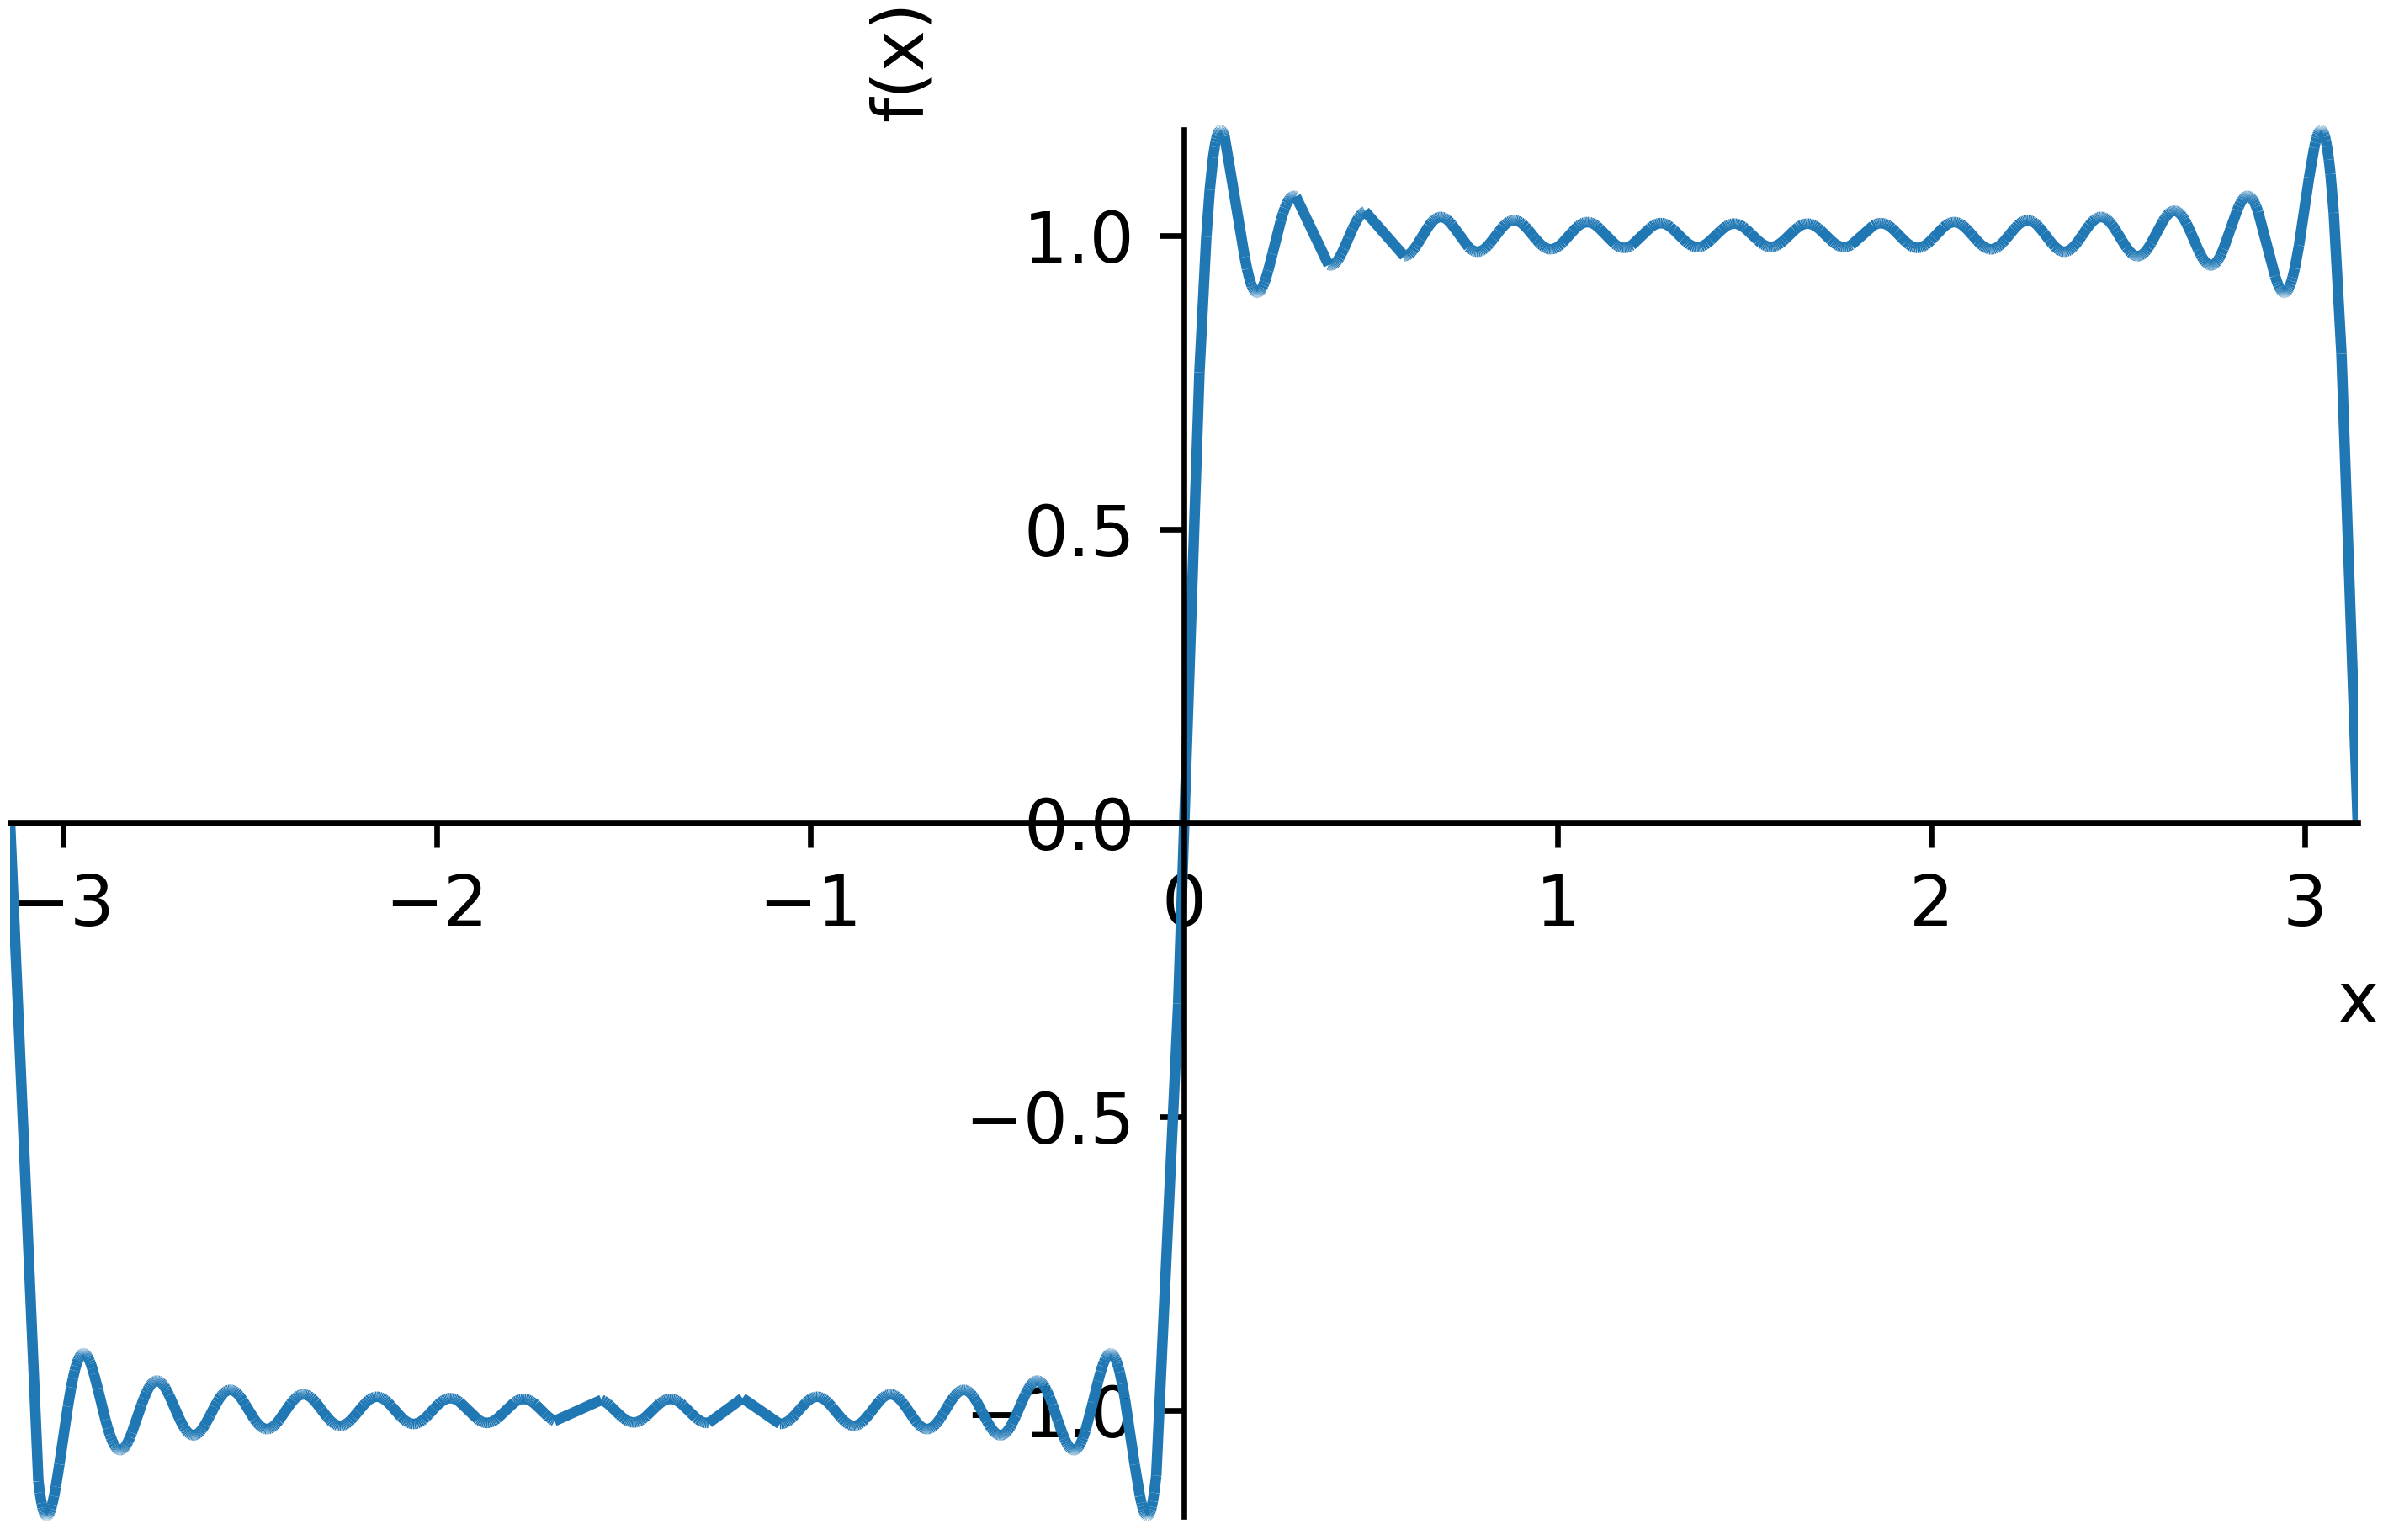
\includegraphics[height=5cm]{fourier.png}
  \end{center}
  \captionsetup{singlelinecheck=off}
  \caption{Lo sviluppo di Fourier della funzione
  che vale $1$ su $[0,\pi]$ e $-1$ su $[\pi,2\pi]$:
  $
  f_{61}(x)=
  \frac{4\sin(x)}{\pi} + \frac{4\sin(3x)}{3\pi} + \frac{4\sin(5x)}{5\pi} + \frac{4\sin(7x)}{7\pi} + \frac{4\sin(9x)}{9\pi} + \frac{4\sin(11x)}{11\pi} + \frac{4\sin(13x)}{13\pi} + \frac{4\sin(15x)}{15\pi} + \frac{4\sin(17x)}{17\pi} + \frac{4\sin(19x)}{19\pi} + \frac{4\sin(21x)}{21\pi} + \frac{4\sin(23x)}{23\pi} + \frac{4\sin(25x)}{25\pi} + \frac{4\sin(27x)}{27\pi} + \frac{4\sin(29x)}{29\pi} + \frac{4\sin(31x)}{31\pi}
  $.
  Il codice per calcolare i coefficienti e generare il grafico
  si trova a pagina~\pageref{code:Fourier}.
  }
  \label{fig:fourier}
  \end{figure}
    
Risulta naturale chiedersi se quella che abbiamo introdotto è una
\emph{base hilbertiana} perché solo in tal caso gli sviluppi di Fourier
approssimano la funzione.
Per ottenere questo risultato dobbiamo assumere la validità del seguente
teorema, che sarebbe ora troppo lungo dimostrare.

\begin{theorem}[densità dei polinomi trigonometrici]
Per ogni funzione continua $f\in C^0([a,b])$
esiste una successione $g_k\in \H(a,b)$ di polinomi trigonometrici
(cioè combinazioni lineari finite del sistema $\ENCLOSE{e_k}$)
tale che $g_k$ converge uniformemente a $f$.

Detto in altri termini: l'insieme dei polinomi trigonometrici
è denso nello spazio $C^0([a,b])$ rispetto alla norma uniforme.
\end{theorem}

Osserviamo che la convergenza uniforme è più forte della convergenza
in $H(a,b)$ in quanto si ha, banalmente:
\[
  \Abs{f}_2^2 = \int_a^b f(x)^2\, dx
  \le \int_a^b \Abs{f}_\infty^2\, dx
  = (b-a) \cdot \Abs{f}_\infty^2.
\]
Dunque il teorema precedente garantisce che ogni funzione continua
in $\H(a,b)$ può essere approssimata, rispetto alla norma $\Abs{\cdot}_2$,
tramite polinomi trigonometrici. Il teorema seguente ci permette
di estendere questa proprietà a tutte le funzioni di $\H(a,b)$.

\begin{theorem}[densità delle funzioni continue]
Data una qualunque $f\in H(a, b)$ per ogni $\eps>0$
esiste una funzione continua $g\colon [a,b]\to \RR$
tale che $\Abs{f-g}_2<\eps$.

Detto in altri termini: $C^0([a,b])$ è un sottospazio denso in $H(a,b)$
cioè un insieme la cui chiusura (nella topologia di $H(a,b)$) è tutto $H(a,b)$.
\end{theorem}
%
\begin{proof}
Se $f\in H(a,b)$ si ha,
per la disuguaglianza di Cauchy-Schwarz:
\[
  \int_a^b \abs{f(x)}\, dx
  \le \Abs{1}_2 \cdot \Abs{f}_2 = \sqrt{b-a}\cdot \Abs{f}_2 < +\infty.
\]
Dunque la funzione $f$ è assolutamente integrabile su $(a,b)$.
Se $f$ è limitata su $(a,b)$ possiamo pensare che $f$ sia definita su $[a,b]$
e l'integrale è un usuale integrale di Riemann (non improprio).
Per le condizioni di integrabilità sappiamo che per ogni $\eps>0$ è possibile
trovare una suddivisione $a=x_0 < x_1 < \dots < x_n =b$ su cui l'integrale
di $f$ differisce dagli integrali superiore e inferiore per meno di $\eps$.
Possiamo prendere come funzione $g$ una interpolazione lineare
cioè una funzione tale che si abbia $g(x_k) = f(x_k)$ sui punti della suddivisione
e che risulti lineare su ogni intervallino $[x_k,x_{k+1}]$. La funzione
$g$ così definita è compresa, su ogni intervallino, tra l'$\inf$ e il $\sup$
di $f$ e dunque si avrà:
\[
 \int_a^b \abs{f(x)-g(x)}\, dx < \eps.
\]
Visto però che $f$ è limitata sappiamo esistere $M>0$ per cui $\Abs{f}_\infty\le M$
e di conseguenza $\Abs{g}_\infty\le M$ e quindi $\Abs{f-g}_2\le 2M$.
Ma allora
\[
  \Abs{f-g}_2^2 = \int_a^b \abs{f(x)-g(x)}^2\, dx
  \le \int_a^b \Abs{f-g}_\infty \cdot \abs{f(x)-g(x)}\, dx
  \le 2M \eps.
\]
Abbiamo quindi mostrato che una funzione limitata e integrabile può essere
approssimata con funzioni continue.

Se la funzione è integrabile in senso improprio su $(a,b)$ ma non è limitata, per
definizione di integrale improprio per ogni $\eps>0$ possiamo trovare un intervallo
$[\alpha,\beta]\subset (a,b)$
per $f$ risulta limitata su $[\alpha,\beta$] e
l'integrale di $f$ su $(a,b)$ differisce dall'integrale di $f$ su $[\alpha,\beta]$
per meno di $\eps$. Ci possiamo quindi ricondurre al passo precedente
per trovare una funzione $g$ che approssima bene $f$ sull'intervallo $[\alpha,\beta]$.
Estendendo $g$ in modo costante su $(a,b)\setminus[\alpha,\beta]$ si troverà
una funzione che approssima bene $f$ su tutto $(a,b)$.
\end{proof}

Grazie ai due teoremi precedenti sappiamo che ogni $f\in \H(a,b)$ può essere
approssimata da polinomi trigonometrici $g_N\to f$
cioè da funzioni della forma:
\[
  g_N = \sum_{k=0}^{N} a_{k,N} e_k.
\]
Stiamo qui assumendo che il polinomio trigonometrico $g_N$ abbia ordine non superiore
ad $N$, ma questo si può sempre assumere, scartando
o ripetendo i termini della successione.

Se ora consideriamo gli sviluppi di Fourier:
\begin{equation}\label{eq:48948784}
  f_N = \sum_{k=0}^N c_k e_k, \qquad c_k = \langle f,e_k\rangle
\end{equation}
ci ricordiamo che per ogni $k\le N$ risulta
\[
   \langle f-f_N, e_k \rangle
   = \sum{k=0}^N \enclose{\langle f,e_k\rangle - c_k} = 0
\]
e quindi
\[
  \langle f-f_N , g_N -f_N\rangle
  = \sum_{k=0}^N \langle f-f_N, (a_{k,N}-c_k) e_k \rangle
  = 0.
\]
Dunque, applicando il teorema di Pitagora,
\[
  \Abs{f-f_N}_2^2 = \Abs{f-g_N}_2^2 - \Abs{f_N-g_N}_2^2
  \le \Abs{f-g_N}_2^2 \to 0.
\]

Abbiamo quindi dimostrato il seguente.
\begin{theorem}[serie di Fourier]
Se $f\in \H(0,2\pi)$ e $c_k$, $f_N$
sono definiti da~\eqref{eq:48948784}
allora $f_k\to f$ in norma $\Abs{\cdot}_2$.
In particolare vale l'uguaglianza di Bessel
\begin{equation}\label{eq:uguaglianza_Bessel}
  \sum_{k=0}^{+\infty} c_k = \Abs{f}_2^2.
\end{equation}
\end{theorem}


Questo significa, dunque, che il sistema ortonormale che abbiamo introdotto
è una base hilbertiana e quindi che ogni funzione $f\in \H(0,2\pi)$
si approssima
rispetto alla norma $\Abs{\cdot }_2$ con gli sviluppi di Fourier.

Ricordiamo che se $\Abs{f_N-f}_2 \to 0$ non è detto che si abbia la convergenza
puntuale $f_N(x)\to f(x)$ per ogni $x\in (0,2\pi)$ in quanto il limite è unico
in $H(a,b)$ ma non in $\H(a,b)$ e dunque è possibile (e in effetti può succedere)
che il limite puntuale degli sviluppi di Fourier differisca, in alcuni punti,
dalla funzione che si sta approssimando.

Purtroppo lo spazio $H(a,b)$ non risulta essere
completo, come si può vedere nel seguente esempio.

\begin{example}[razionali ingrassati]
\label{ex:incompletezza_di_H}%
Dimostrare che lo spazio $H(0,1)$ non è completo.

Sappiamo che l'insieme $[0,1]\cap \QQ$ è numerabile, quindi esiste una
successione $q_k$ che elenca tutti i numeri razionali nell'intervallo $[0,1]$.
Poniamo inoltre $r_k = \frac{1}{4\cdot 2^k}$ e consideriamo gli intervalli
$I_k = [q_k-r_k,q_k+r_k]$.
Prendiamo la successione di funzioni $f_n\colon [0,1]\to \RR$
definita da
\[
  f_n(x) =
  \begin{cases}
  1 &\text{se } x\in\displaystyle\bigcup_{k=1}^{n} I_k\\
  0 & \text{altrimenti}
  \end{cases}
\]
A differenza di quanto uno potrebbe pensare, queste funzioni $f_n$ non diventano
mai identicamente uguali ad $1$. Anzi, si può osservare che
\[
  \int_0^1 f_n(x)\, dx
  \le \sum_{k=1}^n \int_{q_k-r_k}^{q_k+r_k} 1\, dx
  = \sum_{k=1}^n \frac{1}{2\cdot 2^k}
  \le \frac{1}{2}\sum_{k=1}^{+\infty}\frac{1}{2^k} = \frac 1 2.
\]

Si può mostrare che $f_k$ è una successione di Cauchy in $H(0,1)$ e
che però non converge in $H(0,1)$.
\end{example}

\begin{proof}
Per verificare che $f_n$ è una successione di Cauchy possiamo semplicemente
osservare che se $n\ge m$ risulta che $f_n$ e $f_m$ differiscono solamente
sugli intervalli $I_k$ con $k$ compreso tra $m$ ed $n$. Dunque:
\[
  \int_0^1 \abs{f_n - f_m}
  \le \sum_{k=m}^{+\infty} \int_{q_k-r_k}^{q_k+r_k} 1\,dx
  = \sum_{k=m}^{+\infty}\frac{1}{2\cdot 2^k} = \frac{1}{2^m}.
\]
Visto che $f_n$ e $f_m$ assumono solamente i valori $0$ e $1$ anche $\abs{f_n-f_m}$
assume solamente i valori $0$ e $1$ quindi $\abs{f_n-f_m}^2=\abs{f_n-f_m}$.
Abbiamo quindi verificato che per $n\ge m$ si ha:
\[
  \Abs{ f_n - f_m}_2 \le \sqrt{\frac{1}{2^m}}.
\]
E' dunque chiaro che comunque sia scelto $\eps>0$ possiamo scegliere $N$
tale che $1/2^N \le \eps^2$ da cui si ottiene che se $n,m\ge N$
allora $\Abs{ f_n-f_m}_2 \le \eps$. Cioè: $f_n$ è una successione di Cauchy.

Supponiamo ora, per assurdo, che esista $f\in H(0,1)$
tale che $\Abs{ f_n-f}_2 \to 0$.
Innanzitutto visto che ogni $f_k\le 1$ possiamo supporre che sia anche $f\le 1$
perché altrimenti potremmo prendere $g(x) = \min\ENCLOSE{f(x),1}$ e avremmo
chiaramente $\Abs{f_n - g}_2 \le \Abs{f_n -f}_2 \to 0$. In pratica stiamo dicendo
che modificando la funzione $f$ senza cambiarne l'integrale possiamo suppore
che $f(x)\le 1$ per ogni $x\in[0,1]$.

Fissato un intervallo $I_n$, per $k\to +\infty$ si ha:
\[
  0\le \int_{q_n-r_n}^{q_n+r_n}\abs{f_k(x)-f(x)}^2\, dx
  \le \int_0^1 \abs{f_k(x)-f(x)}^2\, dx = \Abs{ f_k -f}_2^2 \to 0.
\]
Ma ora se $k\ge n$ risulta che $f_k=1$ su $I_n$ e quindi il valore dell'integrale
precedente non dipende da $k$ e dovrà quindi essere identicamente nullo:
\[
  \int_{q_n-r_n}^{q_n+r_n} (1-f(x)) \, dx = 0
\]
e quindi possiamo affermare che $\sup f(I_n) = 1$ in quanto se fosse
$\sup f(I_n) = \lambda < 1$
l'integrale di $f(x)-1$ sarebbe positivo
sull'intervallo $I_n$.

Vogliamo ora dimostrare che su ogni intervallo $[a,b]\subset[0,1]$ si ha
$\sup f([a,b])=1$. Prendiamo $N$ abbastanza grande in modo che $r_N < (b-a)/3$.
Allora l'intervallo $[a+r_n, b-r_n]$ ha ampiezza $2 r_n$ e contiene infiniti
numeri razionali. Esistono quindi infiniti indici $n$ per cui $q_n$ sta in tale
intervallo. Tra questi infiniti certamente ce n'è uno con indice $n\ge N$
(perché i $q_n$ con $n< N$ sono in numero finito). Ma se $q_n \in [a+r_n,b-r_n]$
allora $I_n\subset[a,b]$ e quindi $\sup f([a,b])\ge \sup f(I_n) = 1$.

Questo significa che per ogni suddivisione di Riemann dell'intervallo $[0,1]$
risulta che il $\sup$ di $f$ sugli intervallini della suddivisione è $1$ e quindi
l'integrale superiore di $f$ è anch'esso $1$. Dunque, essendo $f$ integrabile,
\[
  \int_a^b f(x) = 1.
\]

Vogliamo ora concludere che questo è in contraddizione con la disuguaglianza
\[
  \int_a^b f_n(x) \le \frac 1 2
\]
che abbiamo osservato all'inizio.
Si ha infatti per la disuguaglianza di Cauchy-Schwarz
\begin{align*}
  \int_0^1 \abs{f(x)-f_n(x)}\, dx
  \le \Abs{f-f_n}_2\cdot \Abs{1}_2  \to 0
\end{align*}
e quindi, per il criterio di convergenza assoluta,
\[
  \int_0^1 (f(x) - f_n(x))\, dx \to 0.
\]
Ma abbiamo visto che
\[
  \int_0^1 (f(x) - f_n(x))\, dx
  = \int_0^1 f(x)\, dx - \int_0^1 f_n(x)\, dx
  \ge 1 - \frac 1 2 = \frac 1 2
\]
ottenendo quindi un assurdo.
\end{proof}

Il fatto di avere trovato una base hilbertiana di $H(0,2\pi)$ (e quindi
in ogni $H(a,b)$) ci permette di
dire che ogni funzione in $H(0,2\pi)$ può essere rappresentata dalle sue
coordinate $c_k$ in modo che valga l'uguaglianza di Bessel:
\[
  \Abs{f}_2 = \sqrt{\sum_{k=0}^{+\infty} c_k^2}.
\]
Abbiamo in effetti definito una corrispondenza:
\[
  \phi \colon H(0,2\pi) \to \ell^2,
  \qquad
  \ell^2=\ENCLOSE{c\in \NN^\RR \colon \sum_{k=0}^{+\infty} c_k^2<+\infty}
\]
definita da
\[
  c_k = \phi(f) = \langle f, e_k\rangle.
\]
Chiaramente tale $\phi$ è lineare. Visto che $e_k$ è una base hilbertiana
è facile verificare che $\phi$ è anche iniettivo. Se su $\ell^2$
definiamo il prodotto scalare e la norma corrispondente:
\[
  \langle x,y\rangle = \sum_{k=0}^{+\infty} x_k y_k, \qquad
  \abs{x}_2 = \sqrt{\sum_{k=0}^{+\infty}} x_k^2
\]
l'uguaglianza di Bessel ci dice che $\phi$ mantiene la norma e quindi
la struttura di spazio euclideo. Si potrebbe dimostrare che $\ell^2$
è completo e questo significa che $\phi$ non è suriettiva in quanto
la successione $f_n$
considerata nell'esempio~\ref{ex:incompletezza_di_H}
è di Cauchy in $H(0,2\pi)$, dunque $\phi(f_n)$ è di Cauchy in $\ell^2$
e dunque converge in $\ell^2$. Il limite $c$ della successione $\phi(f_n)$
rappresenta una successione di coefficienti di Fourier che non possono
essere ottenuti da nessuna funzione $f\in H(0,2\pi)$.

Possiamo utilizzare le serie di Fourier per risolvere 
il seguente\marginnote{%
Il problema di Basilea è un problema posto da Mengoli nel 1650 
e risolto da Eulero nel 1734 dopo che i maggiori matematici del tempo 
(tra cui i famosi membri della famiglia Bernoulli che vivevano appunto a Basilea) 
avevano tentato invano di risolverlo. 
Si tratta di determinare la somma della serie \eqref{eq:basilea}.
La soluzione di Eulero (completamente diversa da quella che stiamo proponendo qui)
è stata poi ripresa da Riemann che ha definito la celebre funzione \emph{zeta}
\index{Riemann!funzione $\zeta$}%
\index{$\zeta$!di Riemann}%
\index{Basilea!problema di}%
\index{problema!di Basilea}%
\index{Eulero!problema di Basilea}%
\index{$\pi$!problema di Basilea}%
\[
\zeta(s) = \sum_{k=1}^{+\infty} \frac{1}{k^s}  
\]
di grandissima rilevanza nella teoria dei numeri.
}.

\begin{exercise}[problema di Basilea]
\label{ex:Basilea}%
Dimostriamo che
\begin{equation}\label{eq:basilea}
  \sum_{k=1}^{+\infty} \frac{1}{k^2} = \frac{\pi^2}{6}.
\end{equation}
\end{exercise}
%%
%%
\begin{proof}[Svolgimento.]
Calcoliamo i coefficienti di Fourier della funzione $f(x)=x$ in $H(0,2\pi)$.
Si ha
\[
 c_0 = \int_0^{2\pi} f(x)\cdot e_0(x)\, dx = \int_0^{2\pi} \frac{x}{\sqrt{2\pi}}\, dx = \frac{1}{\sqrt{2\pi}}\Enclose{\frac{x^2}{2}}_0^{2\pi}
  = \sqrt{2\pi^3}
\]
poi
\begin{align*}
  c_{2k+1} &= \int_0^{2\pi} x \cdot \frac{\sin(kx)}{\sqrt \pi}\, dx \\
   &= \Enclose{\frac{x(-\cos(kx))}{k\sqrt \pi}}_0^{2\pi}
   - \int_0^{2\pi} \frac{-\cos(kx)}{k\sqrt \pi}\, dx\\
   &= \frac{-2\pi}{k\sqrt \pi} - 0 = -\frac{2\sqrt \pi}{k}
\end{align*}
e infine
\begin{align*}
  c_{2k} &= \int_0^{2\pi} x \cdot \frac{\cos (kx)}{\sqrt \pi}\, dx \\
  &= \Enclose{\frac{x \sin(kx)}{\sqrt \pi k}}_0^{2\pi}
  - \int_0^{2\pi} \frac{\sin(kx)}{\sqrt \pi k}\, dx
  = 0.
\end{align*}
Allora l'equazione di Bessel~\eqref{eq:uguaglianza_Bessel} ci dice
che vale
\[
  \Abs{x}_2^2 = \sum_{k=0}^{+\infty} c_k^2
  = c_0 + \sum_{k=0}^{+\infty} c_{2k+1}^2
  = 2\pi^3 + \sum_{k=1}^{+\infty} \frac{4\pi}{k^2}.
\]
Ma è facile calcolare
\[
 \Abs{x}_2^2 = \int_0^{2\pi} x^2\, dx = \Enclose{\frac{x^3}{3}}_0^{2\pi}
  = \frac{8\pi^3}{3}
\]
e quindi
\[
  \frac{8\pi^3}{3} = 2\pi^3 + 4\pi \sum_{k=1}^{+\infty}\frac{1}{k^2}
\]
da cui segue il risultato voluto.
\end{proof}

\section{divagazione sui frattali autosimili}

In questo capitolo mostriamo una applicazione geometrica del teorema delle contrazioni.
Considereremo uno spazio metrico i cui punti sono le figure geometriche
e vedremo che i frattali autosimili non sono altro che punti fissi
di opportune mappe contrattive.

\begin{definition}
Siano $A$ e $B$ sottoinsiemi non vuoti di $\RR^n$.
Definiamo la \emph{distanza di Hausdorff}
\mynote{distanza di Hausdorff}
\index{distanza!di Hausdorff}
tra $A$ e $B$ come:
\[
  d_{\H}(A,B) = \max\ENCLOSE{\sup_{a\in A}\inf_{b\in B} \abs{a-b}, \sup_{b\in B} \inf_{a\in A} \abs{a-b}}.
\]

Definiamo
\[
 \K(\RR^n) = \ENCLOSE{A \subset \RR^n \colon \text{$A$ chiuso, limitato, non vuoto}}.
\]
\end{definition}

\begin{theorem}[caratterizzazione della distanza di Hausdorff]
Se $A$ e $B$ sono compatti di $\RR^n$ (cioè chiusi e limitati) allora
per ogni $r \in \RR$
si ha
\[
  d_\H(A,B) \le r
\]
se e solo se valgono entrambe le seguenti proprietà:
\begin{enumerate}
\item per ogni $a\in A$ esiste $b\in B$ tale che $\abs{a-b}\le r$;
\item per ogni $b\in B$ esiste $a\in A$ tale che $\abs{a-b}\le r$.
\end{enumerate}
\end{theorem}
%
\begin{proof}
Per ogni compatto non vuoto $A$ e per ogni $x\in \RR^n$ definiamo
la distanza tra il punto $x$ e l'insieme $A$ come:
\[
  d(x,A) = \min_{a\in A} \abs{x-a}.
\]
Il minimo esiste in quanto $A$ è compatto e $a\mapsto d(x,a)$ è una funzione continua. Fissato $A$ la funzione $x\mapsto d(x,A)$ è anch'essa continua, anzi è $1$-lipschitziana. Infatti se $x'\in \RR^n$ esiste $a'\in A$ tale che $d(x',A) = d(x',a')$ e dunque
\[
  d(x,A) = \min_{x\in A} \abs{x-a} \le \abs{x-a'} \le \abs{x-x'} + \abs{x'- a'}
   = \abs{x-x'} + d(x',A)
\]
da cui $d(x,A) - d(x',A)\le \abs{x-x'}$.
Scambiando $x$ e $x'$ si ottiene anche la disuguaglianza inversa da cui la $1$-lipschitzianità di $d(x,A)$. Dunque sui compatti la funzione $d(x,A)$ assume sempre massimo e si ha:
\[
d_\H(A,B) = \max\ENCLOSE{\max_{a_\in A} d(a,B), \max_{b\in B} d(b,A)}.
\]

In particolare se $d_\H(A,B) \le r$ per ogni $a\in A$ si deve avere $d(a,B) \le r$ e per ogni $b\in B$ si deve avere $d(b,A) \le r$. Ma allora valgono le due proprietà dell'enunciato.

Viceversa se vale la proprietà 1.\ allora $d(a,B)\le r$ e se vale la 2.\ $d(b,A)\le r$ e di conseguenza $D_\H(A,B) \le r$.
\end{proof}

\begin{theorem}[distanza di Hausdorff]
La distanza di Hausdorff $d_\H$ è una distanza su $\K(\RR^n)$ e lo spazio metrico $\K(\RR^n)$ è completo.
\end{theorem}
%
\begin{proof}
Chiaramente se $A,B$ sono non vuoti si ha $d_\H(A,B) \ge 0$.
Inoltre, in base alla caratterizzazione del teorema precedente è facile osservare che $d_\H(A,B) < +\infty$.

Se $d_\H(A,B) = 0$ significa che per ogni $a\in A$ esiste $b\in B$ tale che $\abs{a-b}=0$. Cioè $b=a$. Dunque $A\subset B$. Scambiando i ruoli di $A$ e $B$ si ottiene anche $B\subset A$ da cui $A=B$.

Che sia $d_\H(A,B) = d_\H(B,A)$ è ovvio in quanto la definizione è simmetrica in $A$ e $B$.

Verifichiamo ora la disuguaglianza triangolare. Siano $A,B,C$ tre compatti non vuoti. Per ogni $a\in A$ esiste $b\in B$ tale che $\abs{a-b} \le d_\H(A,B)$ e per tale $b \in B$ esiste un $c\in C$ tale che $\abs{b-c} \le d_\H(B,C)$. Dunque per ogni $a\in A$ esiste un $c\in C$ tale che
\[
  \abs{a-c} \le \abs{a-b} + \abs{b-c} \le d_\H(A,B) + d_\H(B,C).
\]
Scambiando i ruoli di $A$ e $C$ si ottiene anche la condizione simmetrica e dunque, per la caratterizzazione della distanza di Hausdorff si ottiene la disuguaglianza triangolare:
\[
  d_\H(A,C) \le d_\H(A,B) + d_\H(B,C).
\]

Abbiamo quindi verificato che $d_\H$ è una distanza su $\K(\RR^n)$. Verifichiamo ora che $\K(\RR^n)$ è completo.

Sia $A_k\in\K(\RR^n)$ una successione di Cauchy.
Senza perdita di generalità possiamo supporre che
\[
  d_\H(A_k,A_{k+1}) \le \frac{1}{2^k}.
\]
Infatti essendo $A_k$ di Cauchy è possibile trovarne una sottosuccessione con tale proprietà, e se poi dimostriamo che la sottosuccessione converge allora l'intera successione, essendo di Cauchy, deve convergere.

Consideriamo come candidato limite l'insieme di tutti i possibili limiti di punti degli insiemi $A_k$:
\[
  A = \ENCLOSE{x\in \RR^n
  \colon \exists x_k \in A_k\colon x_k \to x}.
\]

Per prima cosa vogliamo verificare che $A$ non è vuoto. Scelto un punto qualunque $a_0 \in A_0$ esiste $a_1 \in A_1$ tale che $\abs{a_0 - a_1} = d_\H(A_0,A_1)$. Iterando otteniamo una successione di punti $a_k \in A_k$ tale che $\abs{a_k - a_{k+1}} \le d_\H(A_k,A_{k+1}) \le 1/2^k$.
Dunque $a_k$ è una successione di Cauchy in $\RR^n$ ed essendo $\RR^n$ completo dovrà convergere ad un punto $a$ che quindi è un punto di $A$.

Avendo assunto $d_\H(A_k, A_{k+1}) < 1/2^k$ si ottiene (sommando la serie geometrica):
\[
 d_\H(A_k, A_n) \le \sum_{j=k}^{n-1} d_\H(A_j, A_{j+1}) \le \frac{2}{2^k}\qquad \text{se $n>k$}.
\]
Questo ci permette di dimostrare che per ogni $a\in A$ e per ogni $k\in \NN$ esiste $a_k \in A_k$ tale che
$\abs{a - a_k}\le 4/2^k$. Infatti se a distanza $4/2^k$ non ci fossero punti di $A_k$ allora a distanza $2/2^k$ non ci potrebbero essere punti di $A_n$ per nessun $n>k$ in quanto visto che $d_\H(A_k,A_n) \le 2/2^k$ se ci fosse un punto di $A_n$ a distanza inferiore a $2/2^k$ ci dovrebbe anche essere un punto di $A_k$ a distanza inferiore a $4/2^k$. Ma questo è impossibile perché per come è definito $A$ deve esistere $x_n \in A_n$ tale che $x_n \to a$. Abbiamo quindi mostrato che
\[
  \sup_{a\in A} \inf_{b\in A_k} \abs{a-b} \le 4/2^k \to 0.
\]

Viceversa ci proponiamo di mostrare che per ogni $p \in A_k$ esiste $a \in A$ tale che $\abs{p-a} < 2/2^k$.
Visto che $d_\H(A_{j+1},A_j) \le 1/2^j$
possiamo infatti costruire a partire da $a_k=p \in A_k$
una successione $a_j \in A_j$ con $j > k$, tale che $d(a_{j+1},a_j) \le 1/2^j$. Tale successione è di Cauchy
quindi converge: $a_j \to a$
e il suo limite $a$ è quindi un punto di $A$ e si ha
\[
  \abs{a-p} \le \sum_{j=k}^\infty \abs{a_j - a_{j+1}}
    \le \sum_{j=k}^\infty \frac{1}{2^j} \le \frac{2}{2^k}.
\]
Abbiamo quindi dimostrato che
\[
  \sup_{b\in a_k} \inf_{a\in A} \abs{a-b} \le 2/2^k \to 0
\]
e quindi $d_\H(A_k,A)\to 0$.

Ci rimane solo da mostrare che $A$ è un insieme chiuso.
Presa una successione di punti $x_k\in A$ convergente $x_k\to x$, dobbiamo mostrare che $x\in A$. Per ogni $x_k\in A$ per quanto già detto sappiamo esistere $a_k \in A_k$ tale che $\abs{a_k-x_k}\le 4/2^k$. Ma allora $\abs{a_k-a} \le 4/2^k + \abs{x_k-a} \to 0$ e quindi $a_k\to a$ da cui $a\in A$.
 \end{proof}

\begin{theorem}[frattali autosimilari]
Siano $\phi_1, \dots, \phi_N \colon \RR^n \to \RR^n$ contrazioni (cioè funzioni lipschitziane con costante di lipschitz inferiore ad $1$).
Allora
esiste un unico insieme $C\subset \RR^n$ chiuso e limitato tale che
\[
  C = \bigcup_{k=1}^N \phi_k(C).
\]
\end{theorem}
%
\begin{proof}
Basterà dimostrare che la funzione $T\colon \K(\RR^n)\to \K(\RR^n)$ definita da
\[
  T(A) = \bigcup_{k=1}^N \phi_k(C)
\]
è una contrazione: dopodiché sapendo che $\K(\RR^n)$ è completo il risultato è conseguenza diretta del teorema di punto fisso di Banach-Caccioppoli.

Ogni $\phi_k$ per ipotesi è una contrazione, cioè
per ogni $a,b\in X$
\[
  \abs{\phi_k(a)-\phi_k(b)} \le L_k \abs{a-b}
\]
con $L_k< 1$. Posto $L=\max \ENCLOSE{L_1, \dots, L_N} < 1$ vogliamo dimostrare che $T$ è $L$-lipschitziana (e dunque una contrazione). Siano $A,B \in \K(\RR^n)$ e sia $d = d_\H(A,B)$. Preso $a' \in T(A)$ dovrà esistere $k$ tale che $a' \in \phi_k(A)$. Cioè $a'= \phi_k(a)$ con $a\in A$. Ma allora esiste $b\in B$ con $\abs{a-b}\le d_\H(A,B) = d$ e quindi $b'=\phi_k(b) \in T(B)$ e $\abs{a'-b'} = \abs{\phi_k(a)-\phi_k(b)} \le L \abs{a-b} \le L \cdot d$. Dunque abbiamo mostrato che
\[
  \sup_{a' \in T(A)} \inf_{b'\in T(B)} \abs{a'-b'} \le L d_\H(A,B).
\]
La stessa disuguaglianza rimane valida con $A$ e $B$ scambiati, ottenendo quindi:
\[
  d_\H(T(A),T(B)) \le L\cdot d_\H(A,B).
\]
\end{proof}

\begin{example}[insieme di Cantor]
  \label{ex:insieme_Cantor}%
Si prendano $\phi, \psi\colon \RR \to \RR$ definite da
\[
  \phi(x) = \frac{x}{3}, \qquad
  \psi(x) = \frac{2+x}{3}.
\]
Chiaramente $\phi$ e $\psi$ sono $1/3$-lipschitziane e dunque, per il teorema precedente, esiste un unico insieme $C$ chiuso e limitato in $\RR$ tale che
\[
  C = \frac{C}{3} \cup \frac{C+2}{3}.
\]
Tale insieme si chiama \myemph{insieme!di Cantor}.
\index{Cantor!insieme di}

L'insieme di Cantor è un frattale autosimile in quanto si ottiene come l'unione di due copie riscalate di sé stesso.

E' facile mostrare che $C\subset [0,1]$ in quanto $T$ manda sottoinsiemi di $[0,1]$ in sottoinsiemi di $[0,1]$.
Ogni $x\in [0,1]$ può essere rappresentato in base $3$ con una sequenza di cifre ternarie: $0,1,2$. La funzione $\phi(x)$ aggiunge uno $0$ in cima alla sequenza di cifre, mentre la funzione $\psi(x)$ aggiunge un $2$ in cima alla sequenza.
Vogliamo mostrare che $C$ è l'insieme di tutti i numeri in $[0,1]$ che possono essere scritti in base $3$ utilizzando solamente le cifre $0$ e $2$. Osserviamo innanzitutto che $C$ è chiuso: il suo complementare in $[0,1]$ è formato da tutti i numeri che in base $3$ si devono scrivere utilizzando almeno una cifra $1$. Ma se c'è una cifra $1$ posso modificare tutte le cifre successive rimanendo nel complementare di $C$: dunque il complementare di $C$ è aperto. Si osservi che gli unici numeri che hanno una doppia rappresentazione in base $3$ sono quelli che terminano con una sequenza infinita di $2$,
\end{example}

\begin{figure}
\centering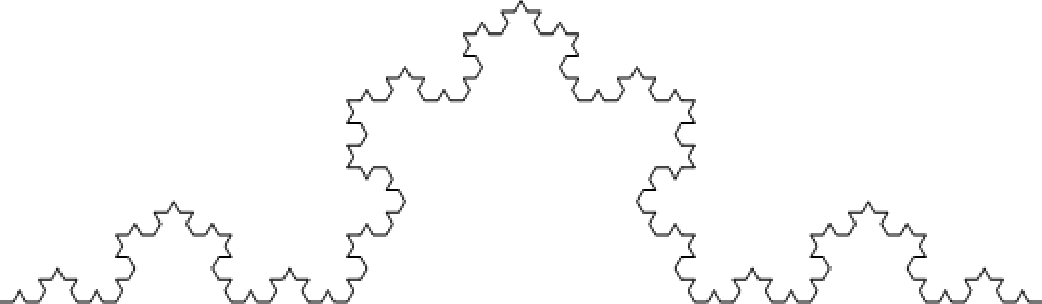
\includegraphics[width=1.0\textwidth]{koch_picture}
\caption{
Chiamato $K_0 \in \RR^2$ il segmento $[0,1]\times \ENCLOSE{0}$,
in figura è rappresentata
la quarta iterata $K_4 = T^4(K_0)$ della contrazione che definisce la curva di K{\"o}ch.
A pagina~\pageref{code:Koch} il codice per generare la figura in copertina.
\index{curva di K{\"o}ch}
}
\label{fig:koch}
\end{figure}

\begin{example}[curva di K{\"o}ch]
Sia $R_\theta\colon \RR^2 \to \RR^2$ la rotazione con centro l'origine di $\theta$ radianti in senso antiorario.
Sia $\alpha = \pi/3$, $p=(1,0)$ e
siano $\phi_1, \phi_2, \phi_3, \phi_4 \colon \RR^2 \to \RR^2$
le funzioni definite da:
\begin{align*}
\phi_1(v) = \frac{v}{3}, \qquad
\phi_2(v) = R_{\alpha}\frac{v}{3} + \phi_1(p), \\
\phi_3(v) = R_{-\alpha}\frac{v}{3} + \phi_2(p), \qquad
\phi_4(v) = \frac{v}{3} + \phi_3(p).
\end{align*}
Allora esiste un unico insieme chiuso $K\subset \RR^2$ tale che
\[
  K = \phi_1(K) \cup \phi_2(K) \cup \phi_3(K) \cup \phi_4(K).
\]
L'insieme $K$ si chiama \myemph{curva di K{\"o}ch}. E' un frattale autosimile in quanto è composto da quattro copie riscalate di se stesso.
\end{example}
